    \documentclass[11pt,a4paper,oneside]{book}

% Include the configuration file for layout.
\usepackage{setspace}
\usepackage{geometry}
\usepackage[toc]{appendix}
\usepackage{lipsum}
\usepackage[export]{adjustbox}
\usepackage[T1]{fontenc}
\usepackage{textcomp}
\usepackage{epsfig,graphics}
\usepackage{graphicx}
\graphicspath{ {./report/assets/} }
\usepackage{titlesec}
\usepackage{amsmath,amsfonts,amssymb,amsthm}
\usepackage{hyperref}
% \usepackage{natlib}
\usepackage[printonlyused,withpage]{acronym}
\usepackage{xcolor}
\usepackage{geometry}
\usepackage{graphicx}
\usepackage{wrapfig}
\usepackage[export]{adjustbox}
\usepackage[section]{placeins}

\usepackage{algorithm}
\usepackage{algorithmic}
\renewcommand{\algorithmicrequire}{\textbf{Input:}}
\renewcommand{\algorithmicensure}{\textbf{Output:}}
\usepackage{amsmath}
\DeclareMathOperator*{\argmax}{arg\,max}
\DeclareMathOperator*{\argmin}{arg\,min}

%%%%%%%%%%%%%%%%%%%%%%%%%%%%%%%%%%%%%%%%%%%%%%%%%%%%%%%%%%%%%%%%%%%%%%%%%%%%%%
% Details of your dissertation
%%%%%%%%%%%%%%%%%%%%%%%%%%%%%%%%%%%%%%%%%%%%%%%%%%%%%%%%%%%%%%%%%%%%%%%%%%%%%%

% Fill in the following fields.
\newcommand{\projectTitle}{Planning to Explore in Reinforcement Learning}
\newcommand{\fullname}{Jared William Swift}
\newcommand{\degreeTitle}{BSc Computer Science with Artificial Intelligence (Ind)}
	% e.g. "BSc Computer Science"
\newcommand{\session}{2022/23}
	% "Session" means the academic year, i.e. 2021/22.
\newcommand{\module}{COMP3931 Individual Project}
	% e.g. "COMP3931 Individual Project".

%%%%%%%%%%%%%%%%%%%%%%%%%%%%%%%%%%%%%%%%%%%%%%%%%%%%%%%%%%%%%%%%%%%%%%%%%%%%%%
% Change the geometry of the page to have a 25 mm binding edge
%%%%%%%%%%%%%%%%%%%%%%%%%%%%%%%%%%%%%%%%%%%%%%%%%%%%%%%%%%%%%%%%%%%%%%%%%%%%%%
 \geometry{
 a4paper,
 total={210mm,297mm},
 left=25mm,
 right=25mm,
 top=25mm,
 bottom=20mm,
 }
 
%%%%%%%%%%%%%%%%%%%%%%%%%%%%%%%%%%%%%%%%%%%%%%%%%%%%%%%%%%%%%%%%%%%%%%%%%%%%%%
% Commands to set the line spacing
%%%%%%%%%%%%%%%%%%%%%%%%%%%%%%%%%%%%%%%%%%%%%%%%%%%%%%%%%%%%%%%%%%%%%%%%%%%%%%
 %\singlespacing
 \onehalfspacing
 %\doublespacing
 
%%%%%%%%%%%%%%%%%%%%%%%%%%%%%%%%%%%%%%%%%%%%%%%%%%%%%%%%%%%%%%%%%%%%%%%%%%%%%%
% Spacing for the chapter header
%%%%%%%%%%%%%%%%%%%%%%%%%%%%%%%%%%%%%%%%%%%%%%%%%%%%%%%%%%%%%%%%%%%%%%%%%%%%%%
 \titleformat{\chapter}[display]
    {\normalfont\Huge\bfseries}{\vspace*{-1\baselineskip}\chaptertitlename\ \thechapter}{15pt}{\huge}
\titlespacing*{\chapter}{0pt}{0pt}{15pt}

\renewcommand\bibname{References}

%%%%%%%%%%%%%%%%%%%%%%%%%%%%%%%%%%%%%%%%%%%%%%%%%%%%%%%%%%%%%%%%%%%%%%%%%%%%%%
% Some shortcuts that maybe useful
%%%%%%%%%%%%%%%%%%%%%%%%%%%%%%%%%%%%%%%%%%%%%%%%%%%%%%%%%%%%%%%%%%%%%%%%%%%%%%
\DeclareTextCommandDefault{\textcopyright}{\textcircled{c}}
 
%%%%%%%%%%%%%%%%%%%%%%%%%%%%%%%%%%%%%%%%%%%%%%%%%%%%%%%%%%%%%%%%%%%%%%%%%%%%%%
% Bibliography style: choose one and make sure you have the relevant .bst file
%%%%%%%%%%%%%%%%%%%%%%%%%%%%%%%%%%%%%%%%%%%%%%%%%%%%%%%%%%%%%%%%%%%%%%%%%%%%%%
\usepackage[square, numbers]{natbib}
% \setcitestyle{square}
% \bibliographystyle{numeric}
\bibliographystyle{plainnat}
% \bibliographystyle{}
%%%%%%%%%%%%%%%%%%%%%%%%%%%%%%%%%%%%%%%%%%%%%%%%%%%%%%%%%%%%%%%%%%%%%%%%%%%%%%
% Layout for the front cover !!!!! YOU SHOULD NOT HAVE TO CHANGE THIS!!!!!
%%%%%%%%%%%%%%%%%%%%%%%%%%%%%%%%%%%%%%%%%%%%%%%%%%%%%%%%%%%%%%%%%%%%%%%%%%%%%%
 
\newcommand{\frontcover}{
% The title page:
\begin{titlepage}
\newgeometry{left=25mm,right=25mm,top=45mm,bottom=0.1cm}

\begin{minipage}[t]{6cm}
\noindent\textbf{\Large{School of Computing}}\\
{\fontfamily{ptm}\selectfont 
\uppercase{faculty of engineering and physical sciences}
}
\end{minipage}
\hfill
\begin{minipage}[t]{7cm}
\vspace*{-15pt}

\includegraphics[scale=0.2,right]{logo_black.png}
\vspace*{-1pt}
\end{minipage}

\noindent\makebox[\linewidth]{\rule{\paperwidth}{0.4pt}}

\centering
\vspace*{20mm}
\textbf{\huge Final Report}\\
\vspace*{20mm}
\textbf{\Large\projectTitle}\\
\vspace*{10mm}
\textbf{\large\fullname}\\
\vspace*{10mm}
\textbf{Submitted in accordance with the requirements for the degree of}\\
\textbf{\degreeTitle}\\
\vspace*{10mm}
\session\\
\vspace*{10mm}
\module\\
\restoregeometry
\end{titlepage}
}

%%%%%%%%%%%%%%%%%%%%%%%%%%%%%%%%%%%%%%%%%%%%%%%%%%%%%%%%%%%%%%%%%%%%%%%%%%%%%%
% Define a new environment for the dissertation summary
%%%%%%%%%%%%%%%%%%%%%%%%%%%%%%%%%%%%%%%%%%%%%%%%%%%%%%%%%%%%%%%%%%%%%%%%%%%%%%
\newenvironment{dissertationsummary}
 	{\cleardoublepage \null 
 		\begin{center}%
			\textbf{Summary}
		\end{center}}%
	{\vfill \null }

\begin{document}
% The prelude is everything up to the start of chapter 1, and is contained
% in a file called "prelude.tex".
\pagenumbering{roman}
\frontcover

\clearpage

\noindent The candidate confirms that the following have been submitted.\\

% Below are examples of what your deliverables may be,
% but since every project is different, not all deliverables
% apply to all projects. Having said that, you should have
% the 'Final Report' deliverable, and most projects will also
% have a link to an online software repository.

\begin{table}[ht!]
\begin{tabular}{|p{0.3\textwidth}|p{0.3\textwidth}|p{0.3\textwidth}|}
\hline 
Items & Format & Recipient(s) and Date \\ 
\hline 
Final Report & PDF file & Uploaded to Minerva (01/05/2023) \\ 
\hline
Link to online code repository & URL & Sent to supervisor and assessor (01/05/2023) \\ 
\hline 
\end{tabular} 
\end{table}


\vfill

\noindent The candidate confirms that the work submitted is their own and the appropriate credit has been given where reference has been made to the work of others.

\vfill

\noindent I understand that failure to attribute material which is obtained from another source may be considered as plagiarism.

\vfill

% Sign this with a pen for all of the hard copies before you hand
% them over to the SSO. If for any reason the submission of final reports
% is online-only, replace the '\rule{}{}' command with your name.
\flushright(Signature of Student) JARED WILLIAM SWIFT
\flushleft

\vfill

\textcopyright~\session~The University of Leeds and~\fullname
% Summary

\begin{dissertationsummary}
Efficient exploration is imperative to success in Reinforcement Learning. However, random approaches, which are not inefficient, are often favoured in practice due to their ease of implementation and robustness. Model-based approaches to exploration are typically more sample efficient, but much of the current approaches are either very optimistic or computationally expensive, and rely on learning a model entirely from scratch and assume that it will eventually become correct.
\newline\newline Within this work we explored a model-based approach to exploration that leverages an initial model, uses a \textit{reasonable} amount of optimism, alongside intrinsic motivation, to explore and learn whilst not assuming that the model will eventually become correct. Exploration was driven by enabling the planner to hypothesise where the model may be incorrect, through additional actions denoted \textit{Meta Actions} and then realising these hypotheses through experience.
\newline\newline Various implementations were developed based on this idea, and were evaluated in a collection of gridworld-like domains, and our method of exploration was shown to perform better than the most ubiquitous random method, $\epsilon$-greedy, in most cases; moreover, the agents with \textit{Meta Actions} available to them often outperformed those without them, showing that they can be a useful exploration mechanism.
\end{dissertationsummary}

\clearpage
\centering\textbf{Acknowledgements}
\flushleft
I'd like to thank my supervisors, Dr. Mehmet Dogar and Dr. Matteo Leonetti, for their constant support and thoughts throughout this project. I'd like to thank Dr. Matteo Leonetti again, for supporting me throughout the entirity of my undergraduate degree, and for providing me with many opportunities to develop autonomous service robotics applications and take part in robotics competitions.
\\I'm grateful for the feedback from my assessor, Dr. Sebastian Ordyniak.
\\I'd like to thank my parents, for everything.


% The contents
\setcounter{tocdepth}{1}
\setcounter{secnumdepth}{4}
\tableofcontents

% The list of figures and tables. Optional.
\clearpage
%\listoffigures
%\listoftables

\pagenumbering{arabic}

 \setlength\parindent{24pt}
% Include as many chapters as you have.
% The "chapter1.tex" etc. files should be in a directory called "chapters"
% \section{List of Acronyms}
% \begin{acronym}
%  \acro{RL}{Reinforcement Learning}
%  \acro{MDP}{Markovian Decision Process}
%  \acro{POMDP}{Partially Observable Markovian Decision Process}
% \end{acronym}



\chapter{Introduction}
\label{chapter1}
Reinforcement Learning (RL) \cite{Sutton1998} is based on the idea of learning through experience; it is trial-and-error learning. A decision-making agent learns how to behave in an environment by interacting with it and receiving positive and negative reinforcement. Experience can only be gained by choosing to try new things and observing the consequences; this is known as exploration. However it's often infeasible to try everything, especially in tasks of practical interest, therefore exploration needs to be done in such a way that it gains maximal knowledge about the environment with minimal learning time and costs \cite{Thrun-1992-15850}. However, the agent also needs to utilise its learned knowledge; this is known as exploitation. This gives rise to the so-called \textit{exploration versus exploitation trade-off}; the agent needs to balance exploration and exploitation in such a way that enables both the acquisition and utilisation of knowledge. Consider a human trying to navigate a maze, as in Figure \ref{fig:maze}. Initially, the human has no knowledge about the maze, so they must choose some path to try; if the path they try is realised to lead to a dead end, they might receive some negative reinforcement, and learn that this path is not a good one to take. To escape the maze, the human must try new things; they must explore the maze and discover where the dead ends are, and which paths seem promising, but they also need to exploit the knowledge that they have gained, and follow the promising paths. 
\\Conversely to RL, Automated Planning (or just Planning) \cite{GhallabNauTraverso04, Lav06, DBLP:books/aw/RN2020} uses embedded knowledge of the environment, in the form of a model, to determine the optimal sequence of successive actions to fulfil a given goal. However, planning relies on the model to accurately represent the environment; which cannot be guaranteed, due to approximations, abstractions, and human-error, and therefore planning can be quite fragile. As an example, consider Figure \ref{fig:maze} again. Imagine the human is given a map of the maze, but it shows the true path out of the maze to be a dead end. The human might look at the map and decide it's impossible to escape the maze.
\\Planning and RL take different approaches to decision-making; relying on previously obtained, or embedded, knowledge versus obtaining knowledge through experience. However, they may be combined, which is known as Model-Based RL (MBRL); which is most commonly encapsulated in the form of planning over a learned model, which has been shown to be very effective in recent years \cite{silver2017mastering, pmlr-v28-levine13}. Coming back to the example in Figure \ref{fig:maze}, the human could reason to try the true path that seems like it is a dead end, and realise that it is not actually a dead end, and update the map for the next person.
\\ Exploration is a widely studied topic in RL, since it necessitates learning. Thus, strategies for exploration vary widely. A particularly interesting avenue of research is the use of models within exploration - from using approximate models to constrain exploration, such as DARLING \cite{AIJ16-leonetti}, to using optimistic models to guide exploration, such as OIM \cite{10.1145/1390156.1390288}, to using ensembles of models to derive novel states to explore towards, such as MAX \cite{DBLP:journals/corr/abs-1810-12162}. In practice, however, model-free exploration methods based on randomness, such as $\epsilon$-greedy \cite{conf/nips/Sutton95, Watkins:1989} are ubiquitous.
\\Exploration in RL is still an open problem; many advanced, complex, techniques have been proposed, but the most widely used techniques remain the simplest. Thus, within this work we explore the development of a framework that synergises planning and
learning in order to drive exploration by making intelligent hypotheses about the
environment, informed by the inherently inaccurate, but still useful, model, previous experience
and environmental observations, with the goal being to mitigate model inaccuracies on the quality of learned behaviour, and an overarching aim of distancing the field of exploration from randomness.

% The ultimate goal of this
% work is to mitigate the effect of the inherent inaccuracies in the model on the quality of learned
% behaviour; resulting in agents that can learn beyond the inaccuracies of the model, through
% intelligent exploration.

\begin{figure}[h!]
    \centering
    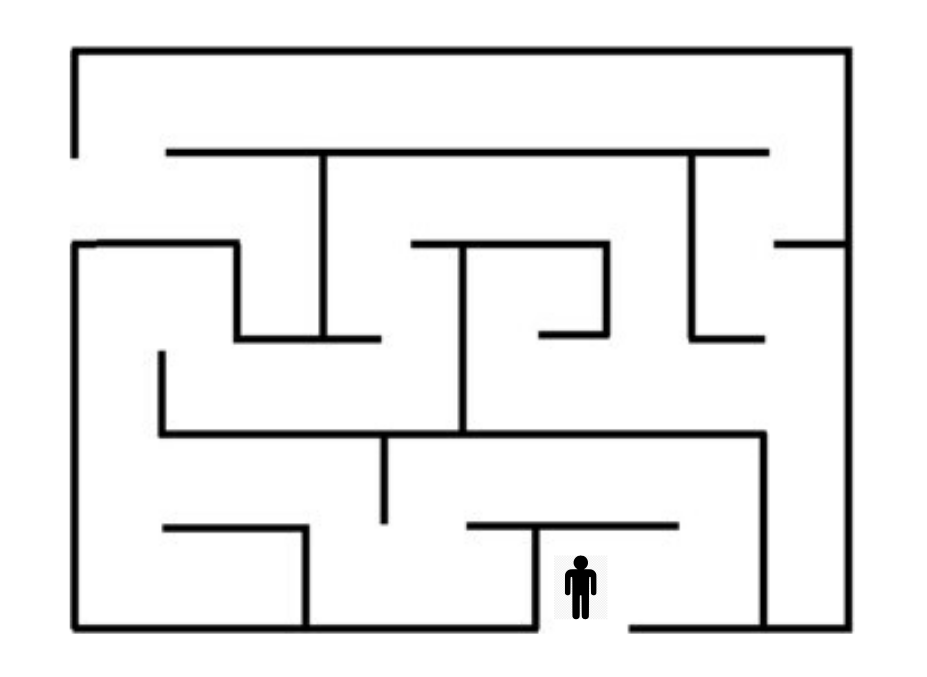
\includegraphics[max size={350pt}{350pt}]{report/assets/maze.png}
    \caption{Maze Navigation}
    \label{fig:maze}
\end{figure}
\chapter{Background Research \& Notation}
\label{chapter2}
Within this chapter, we begin by introducing the formal method for representing sequential decision making problems. We then proceed to formally introduce Planning and discuss some algorithms of interest. We finish by formally introducing Reinforcement Learning, the various encapsulations of RL and providing a short survey of exploration methods in RL; this survey is the main bulk of our literature review.
\section{Markov Decision Processes}
The Markov Property states that the future is conditionally independent of the past given the present. A sequential decision-making problem that satisfies the Markov Property is known as a Markov Decision Problem, and can be modelled by a Markov Decision Process (MDP) \cite{10.5555/528623}. Where an agent is able to fully observe its state, the problem can be modelled as an MDP. Conversely, where an agent can only partially observe its state, the problem can be modelled by a Partially Observable Markov Decision Process (POMDP).
Consider an agent playing a perfect information game, such as Chess or Go, the agent (and its opponent) are able to fully observe the state of the game with ease. However, a robot navigating through a maze may not be able to observe its exact state due to uncertainty in its sensors.
Furthermore, an MDP can be stationary or non-stationary which refer to whether its dynamics stay the same, or change temporally.
An MDP that contains absorbing states, that is any state that upon entering the task terminates, then is said to be episodic.
\\Within this work we assume that the agent is fully able to observe its state, the environment is stationary and can be discretised in some way and tasks are episodic.
Hence we consider \textbf{stationary}, \textbf{finite}, \textbf{undiscounted} MDPs.
Thus, an MDP is a 4-tuple, $\text{MDP} = (S,A,T,R)$ where:
\begin{itemize}
    \item $S$ is a finite set of states.
    \item $A$ is a finite set of actions.
    \item $T : S \times A \times S \rightarrow [0,1]$ is the transition function, which determines the probability of transitioning from a state $s \in S$ to $s' \in S$ with an action $a \in A$.
    \item $R:S \times A \times S \rightarrow \mathbb{R}$ is the reward function, which determines the reward signal, $r \in \mathbb{R}$ received by the agent from transitioning from a state $s \in S$ to $s' \in S$ with the action $a \in A$. This reward is extrinsic to the agent; it comes from the environment.
\end{itemize}
\begin{defn}
\label{defn:determinism}
An MDP is said to be deterministic if $\forall s,s' \in S, \forall a \in A$, $T(s,a,'s) \in \{0,1\}$.
\end{defn}
\begin{defn}
\label{defn:stochastic}
An MDP is said to be stochastic if it is not deterministic
\end{defn}
\subsection{Policies, Value and Quality}
A policy, denoted by $\pi$, is a mapping of states to actions that describes a behaviour within an MDP. The desired behaviour within an MDP is to maximise the cumulative reward, this is known as the optimal policy and denoted $\pi^*$. The cumulative reward is given by:
\begin{equation}
\label{eqn:return}
G_t = \sum_{k=t+1}^TR_{k}
\end{equation}
which represents the cumulative reward received from time $t$ to some finite time $T$.
A Value Function, or state-value function, denoted $V^\pi(s)$, measures the expected cumulative reward that can be received starting in each state $s \in S$ and following a policy $\pi$:
\begin{equation}
\label{eqn:vs}
    V^\pi(s) = \mathbb{E}^\pi\Bigg[G_t | s_t = s\Bigg] = \mathbb{E}^\pi\ \Bigg[\sum_{k=t+1}^TR_{k} | s_t = s \Bigg]
\end{equation}
Where $\mathbb{E}$ represents the expected value that the agent follows $\pi$, $t$ is an arbitrary time step and $T$ is a finite time horizon.
The optimal Value Function, $V^*$, is the one that is maximum for every $s \in S$ and is given by:
\begin{equation}
\label{eqn:vsm}
     V^*(s) = \max_\pi V^\pi(s) 
\end{equation}
This can also be represented in a recursive form, known as the Bellman Optimality equation for $V$:
\begin{equation}
\label{eqn:vsB}
V^*(s) = \max_a\sum_{s'}T(s,a,s')[R(s,a,s')+V^*(s')]
\end{equation}
Similarly, a Q-Function, or action-value function, denoted $Q^\pi(s,a)$, measures the expected cumulative reward that can be received starting in each state $s \in S$, taking an action $a \in A$ and thereafter following a policy $\pi$:
\begin{equation}
\label{eqn:qsa}
Q^\pi(s,a) = \mathbb{E}^\pi\Bigg[G_t | s_t = s,a_t = a\Bigg] = \mathbb{E}^\pi\Bigg[\sum_{k=t+1}^TR_{k}|s_t=s, a_t = a\Bigg]
\end{equation}
Where $\mathbb{E}$ represents the expected value that the agent follows $\pi$, $t$ is an arbitrary time step and $T$ is a finite time horizon.
The optimal Q-Function, $Q^*$, is the one that is maximum for every $s,a \in S \times A$ and is given by:
\begin{equation}
\label{eqn:qso}
Q^*(s,a) = \max_\pi Q_\pi(s,a)
\end{equation}
Similarly to the Value Function, this can also be represented in a recursive form, known as the Bellman Optimality equation for $Q$:
\begin{equation}
\label{eqn:qsB}
Q^*(s,a) = \sum_{s'}T(s,a,s')[R(s,a,s')+\max_{a'}Q^*(s',a')]
\end{equation}
An interesting observation is that $\pi^*$ can be derived from both $V^*$ and $Q^*$. In the case of $V^*$, $\pi^*$ can be derived by determining at each state, which actions yield the next state with the maximum value. In the case of $Q^*$, $\pi^*$ can be derived by simply taking the action with the highest Q-value at each state \cite{Sutton1998}.

\section{Planning}
Planning involves reasoning on a model of an environment, in order to produce a sequence of successive actions that will achieve a specified goal whilst satisfying some constraints or achieving some objectives, such as minimising cost \cite{GhallabNauTraverso04, Lav06, DBLP:books/aw/RN2020}.
\\In the context of MDPs, the goal is to maximise cumulative reward. Formally, let $s_t \in S$ be some start state at a discrete time, $t$. The goal of the planner is to produce a sequence of actions, $P=(a_t, a_{t+1},...,a_{t+n})$, such that $\pi^*(s_t) = P(t)$, for all $t$.
% \\Formally, the goal of Planning is given an MDP, $M$, start and goal states, $s$ and $g$, to produce a sequence of actions, $P=(a_0, a_1,...,a_n)$, such that executing $P$ would result in transitioning from the start state to the goal state.
\\Planning has been a widely studied topic in AI for many years and as such there exist many planning methods and algorithms. While the use of Planning is central to this work, particular planning methods and algorithms are not; therefore, we only consider heuristic search methods and planning by Dynamic Programming.
\subsection{Heuristic Search}
Heuristic search (or informed search) \cite{EdelkampSchroedl11} is a class of search algorithms that use problem specific knowledge in the form of heuristics to guide the search. A heuristic, denoted $h(s)$, is a function that estimates the cost of transitioning from the current state, $s$, to the goal state. We consider best-first search algorithms, which aim at expanding states that appear best according to an evaluation function, denoted $f(s)$. 

\subsubsection{A* Search}
\label{sec:astar}
A* Search (or just A*) \cite{4082128} is a heuristic search algorithm that is a form of best-first search. A cost function, $g(s)$, is introduced, which indicates the cost to get from the start state to a state $s$. The main idea is that the evaluation function can be a combination of the cost to get to the state being evaluated, $g(s)$, and the estimated cost to get from the state being evaluated to the goal state, thus:
\begin{equation}
\label{eqn:astarr}
f(s) = g(s) + h(s)
\end{equation}
The evaluation function indicates the estimated cost of the minimum cost solution that passes through $s$ \cite{DBLP:books/aw/RN2020}. A* works by guiding the search to expand states with the lowest value for $f(s)$ first, in order to determine a sequence of states which is the path (or in our case, the plan). A* is a complete algorithm; it will always find a solution if one exists. However, the optimality of A* depends on the choice of the heuristic: the heuristic must be admissible, which means that it must never overestimate the cost of getting from the current state to the goal state; in this sense, the heuristic must always be optimistic.

\subsection{Dynamic Programming}
Dynamic Programming (DP) \cite{Bellman:1957, DBLP:books/lib/Bertsekas05} refers to a collection of methods that can be used to solve MDPs, by computing the optimal policy with respect to them. The two main algorithms that we consider are Policy Iteration and Value Iteration; both of which are forms of Generalised Policy Iteration (GPI). GPI refers to any process that involves Policy Evaluation and Policy Improvement acting with each other. As it happens, most DP and RL methods are forms of GPI \cite{Sutton1998}.

\subsubsection{Policy Evaluation and Improvement}
Given a policy, $\pi$, it can be evaluated by computing its Value Function, $V^\pi$:
\begin{equation}
\label{eqn:policyeval}
V^\pi = \sum_a \pi(a|s)\sum_{s'}T(s,a,s')[R(s,a,s') + V^\pi(s')]
\end{equation}
Policy Improvement is the process of generating an improved policy from a suboptimal policy \cite{DBLP:books/lib/Bertsekas05}. A policy $\pi$ could be improved by contemplating taking an action $a \in A$ in a state $s \in S$, such that $\pi(s) \neq a$ and then continue following $\pi$ thereafter. We can evaluate this change by computing the Q-function for $s,a$:
\begin{equation}
\label{eqn:qval}
Q^\pi(s,a) = \sum_{s'}T(s,a,s')[R(s,a,s') + V^\pi(s')]
\end{equation}
Then comparing $Q^\pi(s,a)$ with $V^\pi(s)$. If $Q^\pi(s,a) > V(s)$, then the policy is update and improved as such: $\pi(s) = a$.
\subsubsection{Policy Iteration}
Policy Iteration (PI) \cite{Bellman:1957, howard:dp} is a method for computing the optimal policy of an MDP. Assuming an arbitrary initial policy, $\pi$, at each step $\pi$ is evaluated, yielding a Value Function $V^\pi$ (or a Q-Function $Q^\pi$). The policy is then updated greedily with respect to $V^\pi$ (or $Q^\pi$). This iterative process leads to monotonic improvements to $\pi$.
\subsubsection{Value Iteration}
Value Iteration (VI) \cite{Bellman:1957} is a method for computing the optimal estimate for the Value or Q-Function of an MDP. As the estimate approaches optimality, the policy that is greedy with respect to the Value or Q-Function also approaches optimality \cite{series/synthesis/2010Szepesvari}.
In the context of Value Functions, assuming an arbitrary initial estimate, $V$, at each step $V$ is updated as such:
\begin{equation}
\label{eqn:vupdate}
V(s) = \max_a\sum_{s'}T(s, a, s')[R(s, a, s')+V(s')]
\end{equation}
for all $s \in S$. This update originates from the Bellman optimality equation for $V$, Equation \ref{eqn:vsB}.
For Q-Functions, assuming an arbitrary initial estimate, $Q$, at each step $Q$ is updated as such:
\begin{equation}
\label{eqn:qupdate}
Q(s,a) = \sum_{s'}T(s,a,s')[R(s,a,s') + \max_{a'}Q(s',a')]
\end{equation}
for all $s \in S$, $a \in A$. This update originates from the Bellman optimality equation for $Q$, Equation \ref{eqn:qsB}.

\section{Reinforcement Learning}
Within an RL setting, formalised by an MDP, an agent learns how to behave in an environment by interacting with it through actions, at discrete, sequential, time steps, and observing the affects through its new state and a scalar reward signal, as seen in Figure \ref{fig:rl}. The reward signal may be delayed, meaning that the consequences of actions may not be known until long after they are taken \cite{barto1990learning}. This gives rise to the (temporal) credit assignment problem \cite{Minsky:1961:ire}, the problem of determining which actions led to an outcome and assigning credit among them; it's often the case that a sequence of actions led to an outcome, rather than a single action. The ultimate goal of the agent is to learn a policy, $\pi^*$, that maximises the expected cumulative long-term reward \cite{Sutton1998}; as we outlined in Chapter \ref{chapter1}, exploration, exploitation and the trade-off between the two, are key to this. The two main instantiations of RL are model-free and model-based, each of which we will delve deeper into within this section.
\begin{figure}[h!]
    \centering
    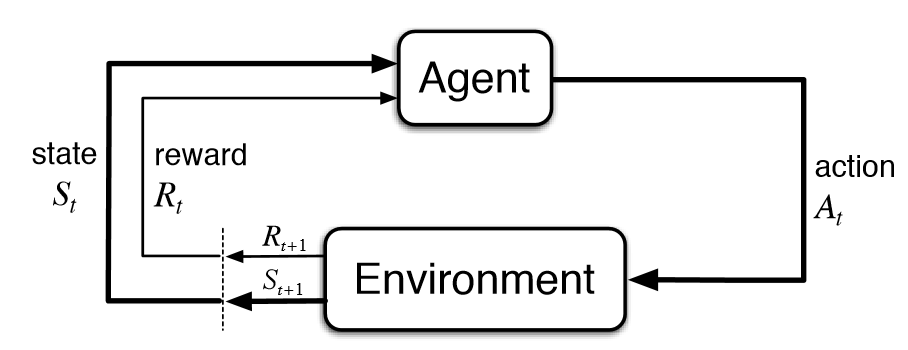
\includegraphics[max size={325pt}{325pt}]{report/assets/rl.png}
    \caption{The RL Loop \cite{Sutton1998}}
    \label{fig:rl}
\end{figure}

\subsection{Model-free RL}
Model-free (or direct) is where the agent learns a policy directly from experience gained by interacting with the environment; it is purely trial-and-error. Model-free learning tends to be quite flexible to varying problems, since no assumptions are made about the environment's dynamics. Furthermore, since the environment's dynamics do not need to be stored, learned or considered, model-free learning is scalable and does not suffer from the \textit{curse of dimensionality} (in the non-tabular cases) and can be computationally efficient, as there is generally no lookahead deliberation process involved. However, model-free learning can be sample-inefficient; the agent may need to take many actions before discovering the optimal policy. Moreover, in real-world domains, model-free learning may not even be feasible, due to the cost of experience. The most common model-free approach is Temporal Difference Learning.

\subsubsection{Temporal Difference Learning}
Temporal Difference (TD) Learning \cite{10.5555/911176, 5392560, 5391906} aims at solving the problem of temporal credit assignment by combining ideas from Monte Carlo methods, which learn directly from experience in the environment, and Dynamic Programming methods, which bootstrap estimates from other previously learned estimates; it is a form of GPI \cite{Sutton1998}.
% It is a form of Generalised Policy Iteration, in that it aims to produce an optimal estimate of the Value Function, $V_\pi^*$, starting from an initial estimate, $V_\pi$, for a given policy, $\pi$,\cite{Sutton1998}.
\\The core idea of TD Learning is to update the estimate of the Value Function, $V_\pi$, whenever there is a difference between temporally successive predictions. This difference is known as the TD error. The updated estimate is bootstrapped from the previous estimate, meaning that TD learning essentially learns a prediction from another prediction.
\\The simplest TD Learning algorithm is TD(0), which updates it's estimates as such:
\begin{equation}
\label{eqn:td0update}
V(s_t) = V(s_t) + \alpha[r_{t+1} + V(s_{t+1}) - V(s_t)]
\end{equation}
The TD target is the current prediction of the expected cumulative reward: $r_{t+1} + V(s_{t+1})$, the TD error is $r_{t+1} + V(s_{t+1}) - V(s_t)$ and $0 \le \alpha \le 1$ is the learning rate, which is used to control how much weight is given to the TD error when updating the estimate \cite{Sutton:1988}.
\\TD Learning can also be extended to learn a Q-Function, which stores the value of state-action pairs rather than the value of states. For each state-action pair, it stores an estimate of the expected cumulative reward starting in that state and taking an action, and following a fixed policy. This can be done using Q-Learning and SARSA.

\paragraph*{Q-Learning} \cite{Watkins:1989, journals/ml/WatkinsD92} is an off-policy TD Learning method that learns a Q-function. It is off-policy, as the update rule assumes a greedy policy - this means that the value of the optimal policy is learned independently of the agent's actions following the current policy. Q-values are iteratively updated using the Bellman equation, the update rule is as follows:
\begin{equation}
\label{eqn:qlearningupdate}
Q(s_t,a_t) = Q(s_t,a_t) + \alpha[r_{t+1} + \max_aQ(s_{t+1}, a) -Q(s_t,a_t)]
\end{equation}
\paragraph*{SARSA} (State Action Reward State Action) \cite{rummery:cuedtr94} is an on-policy TD Learning method that learns a Q-function. It is on-policy, as the update rule assumes that the current policy continues being followed - this means that the value of the current policy being followed is learned. Q-values are iteratively updated using the Bellman equation, the update rule is as follows:
\begin{equation}
\label{eqn:sarsaupdate}
Q(s_t, a_t) = Q(s_t, a_t) + \alpha[r_{t+1} + Q(s_{t+1}, a_{t+1})-Q(s_t, a_t)]
\end{equation}

\subsection{Model-Based Learning}
Model-based (or indirect) RL is where an agent uses a known or learned model of the environments dynamics (in the form of an MDP) in order to learn an optimal policy. The agent may learn the model and policy at the same time, as in the Dyna family \cite{Sutton:1990, 10.1145/122344.122377} or learn a policy by planning over a known model, as in AlphaZero \cite{DBLP:journals/corr/abs-1712-01815} or learn a policy by planning over a learned model, as in MuZero \cite{DBLP:journals/corr/abs-1911-08265}. Model-based RL offers improved real-world sample efficiency, potential for directed, informed exploration and better asymptotic performance, the prospect of transfer learning, safer learning and explainability \cite{MAL-086}. These benefits come at a computational cost, typically in planning; however we take the stance that this added computational cost is certainly worth it, particularly for the benefit of reducing learning costs. 
Since it's not always the case that a model is known as a priori, and even if it is it might be inaccurate, model-learning is a key component of model-based RL.

\subsubsection{Model Learning}
Model Learning can be difficult due to uncertainty caused by limited data and stochasticity. Uncertainty can be overcome through sufficient exploration; sampling a transition multiple times can give a better estimate of its probability distribution.
\\Model learning can be viewed as a supervised learning problem \cite{JORDAN1992307}. In discrete environments, exact models of the environment's dynamics can be learned in the form of a \textit{tabular maximum likelihood model} \cite{10.1145/122344.122377} which  maintains a table with an entry for every possible transition.
In the stochastic case, for each transition the table will store:
\begin{equation}
\label{eqn:tmlmupdate}
T(s, a, s') = \frac{n(s, a, s')}{\sum_{s'}n(s,a,s')}
\end{equation}
Where $n : S \times A \times S \rightarrow \mathbb{Z}$ represents the number of times a transition has been observed. This also works for the deterministic case, which will result in all transitions mapping to either 0 or 1; but this leads to unnecessary computations; it's better to manually update $T$ if the domain is known to be deterministic.
A key drawback to this approach is the lack of scalability to large state spaces.
\\In continuous domains an exact model cannot be learned, due to the infinite number of states (and potentially actions). An approximate model can be learned by using state aggregation (which discretises the state space) and a tabular maximum likelihood model \cite{Kuvayev1996ModelBasedRL}.
\\In continuous domains its impossible to learn an exact tabular model, and it may also be infeasible for discrete domains with large state spaces, therefore an approximate model must be learned; most commonly this is done through Function Approximation methods, such as Linear Regression \cite{DBLP:journals/corr/abs-1206-3285, NIPS2007_b7bb35b9} and Gaussian Processes \cite{10.5555/3104482.3104541}.

\section{Exploration Methods in Reinforcement Learning}
Within this section, we will provide a brief survey of exploration methods in RL. Whilst Thrun distinguished between undirected and directed exploration \cite{Thrun-1992-15850}, and Amin et al. distinguished between reward-free and reward-based exploration \cite{DBLP:journals/corr/abs-2109-00157}, there is no definitive taxonomy of exploration methods; as such, we will use our own categories, which distinguishes between model-free, model-based and hybrid approaches.
\subsection{Model-Free Methods}
Model-free exploration methods are characterised by the fact that they do not use, or learn, a model to aid exploration. This means that they can be robust to varying domains, where designing or learning a model could prove difficult. However, they must rely on other methods to drive exploration, which tend to be grounded in randomness.
\\Purely random exploration comes in the form of a Random Walk, or unguided random search \cite{anderson86}, which arises from randomly sampling actions with uniform probability. Exploration occurs naturally when the agent moves away from the goal, rather than closer to it. This is perhaps the most naive exploration method, since it is entirely random, and thus it is very inefficient and rarely used in practice.
\\ Boltzmann exploration samples an action according to the Boltzmann distribution:
\begin{equation}
\label{eqn:boltzmann}
\pi(a|s) = \frac{e^{Q(s,a)/\tau}}{\sum_{a' \in A}e^{Q(s,a')/\tau}}
\end{equation}
Where the temperature, $0 \le \tau \le 1$, is a hyperparameter that determines how frequently random actions are chosen; as $\tau$ approaches 0, the policy approaches greediness \cite{Thrun-1992-15850, DBLP:journals/corr/abs-2109-00157}. When there are large differences between Q-values, little exploration occurs, however when Q-values are close to each other, considerable exploration occurs. This means that Boltzmann exploration has a particular reliance on the initialisation of the Q-values, and the early exploration \cite{wiering}. Moreover, Boltzmann exploration does not consider uncertainty in Q-values \cite{DBLP:journals/corr/Cesa-BianchiGLN17}, which can lead to actions being chosen which appear to be promising, but in reality are not, due to epistemic uncertainty. 
% Various modifications have been suggested to Boltzmann exploration to overcome its problems, such as using learning-rate schedules to attenuate the temperature \cite{singh00} and per-action learning rates \cite{DBLP:journals/corr/Cesa-BianchiGLN17}.
\\$\epsilon$-greedy \cite{Watkins:1989, conf/nips/Sutton95} uses a hyperparameter, $0 \le \epsilon \le 1$ to explicitly balance between exploration and exploitation. With probability $\epsilon$ the agent explores by taking a random action, which is sampled with uniform probability, with probability $1-\epsilon$ the agent exploits by taking the best action, which is selected greedily with respect to the current policy. Uniformly choosing actions means that actions which are known to be sub optimal can be continually evaluated long after they are realised to be so.
\\Pure random exploration is very inefficient, and certainly not a practical exploration method. Boltzmann exploration and $\epsilon$-greedy offer better exploration strategies than pure randomness, but they are not without their faults. Moreover, model-free methods in general tend to lack temporal persistence which can lead to indecisiveness during exploration, for instance moving back and forth between two states, leading to inefficient exploration. Extensions have been proposed to Boltzmann exploration and $\epsilon$-greedy that overcome some of their respective issues, such as Boltzmann-Gumbel exploration \cite{DBLP:journals/corr/Cesa-BianchiGLN17} and $\epsilon z$-greedy \cite{dabney2021temporallyextended}, although the standard methods seem to favoured in practice.
%  h e Boltzmann rule causes a lot of exploration in states where Q-values for different
% actions are almost equal, and little exploration in states where Q-values are very different.
% This is helpful for risk minimization purposes (Heger, 1994), for which we may prefer not
% to explore actions which look significantly worse t h a n others. However, initially learned Q-
% estimates can be incorrect due to noise, so some exploration is still needed in case of large
% differences in Q-values. Using an annealing schedule for the t e m p e r a t u r e should get around
% this problem, b u t finding a good annealing schedule can be quite difficult and is reward
% function dependent.2 Furthermore, since the t e m p e r a t u r e is a global variable, it may happen
% t h a t some state is not visited for a long time, after which the amount of exploration in
% this state is very small. Although this last problem could be solved using local t e m p e r a t u r e
% variables, it is still a problem t h a t the agent may concentrate on different trajectories which
% it already knows well.


% \\ Pure random exploration is extremely inefficient, and will likely not succeed in complex domains. Boltzmann exploration and $\epsilon$-greedy offer a stronger solution than pure randomness, but they still have their respective limitations, which can lead to getting stuck in a local optima.

% While model-free exploration methods can be robust and applicable to a wide range of domains, they also come with some weaknesses. Random exploration can be highly inefficient and often fails to achieve the exploration goals within reasonable time constraints. Boltzmann exploration and ε-greedy methods are more efficient than random exploration, but they still have limitations. Boltzmann exploration may not work well in environments where the optimal action is much better than the suboptimal ones, as it may lead to the agent choosing suboptimal actions too often. Similarly, ε-greedy methods may not be effective in environments where there are many equally good actions, as the agent may get stuck in a suboptimal action instead of exploring all possible options. Therefore, while these methods have their advantages, it is important to consider their limitations and choose the exploration strategy that is best suited to the particular domain and task at hand.

% Whilst Boltzmann Exploration and $\epsilon$-greedy are simple exploration strategies that are very commonly used in practice, they suffer from a variety of issues. Firstly, there is no temporal persistence. There is als
% \\ Boltzmann Exploration and $\epsilon$-greedy are very commonly use exploration methods in practice.
\subsection{Model-Based Methods}
Model-based exploration methods are those that use, or learn, a model to drive exploration.
\subsubsection{Optimistic}
Optimistic exploration methods are based on the \textit{optimism in the face of uncertainty} (OFU) principle \cite{DBLP:journals/corr/cs-AI-9605103}.
\\Explicit, Explore or Exploit ($E^3$)  \cite{Kearns+Singh:2002} maintains a partial model of the environment through collecting statistics, akin to the \textit{tabular maximum likelihood} approach. A distinguishment is made between \textit{known} and \textit{unknown} states; a state is \textit{known} after it has been visited an arbitrary number of times, thus its learned dynamics must be close to the true dynamics. If the current state is \textit{unknown}, then \textit{balanced wandering} takes place, and the agent explores by selecting the action that has been taken the least number of times from that state. If the current state is \textit{known}, then an exploitation policy and an exploration policy are computed. One of these policies is chosen and followed for a finite time horizon; exploitation is chosen if the policy will induce large cumulative reward, exploration is chosen otherwise.
\\ R-MAX \cite{10.1162/153244303765208377} is an extension and generalisation of $E^3$. It begins with an optimistic initial model such that every transition leads to some imaginary state, \textit{The Garden of Eden State}, that returns the maximal reward, denoted $R_{max}$. R-MAX uses the same concept of \textit{known} and \textit{unknown} states as in $E^3$; after a state becomes known, then the model is updated with the collected statistics regarding that state. The agent always follows the optimal policy according to the model. R-MAX removes the need for explicit contemplation between exploring and exploiting as in $E^3$; exploration and exploitation occur naturally.
\\ Optimistic Intial Model (OIM) \cite{10.1145/1390156.1390288} begins with an optimistic model, the same as R-MAX. The model is updated through observations similarly to $E^3$. The agent maintains two Q-functions; one for the real extrinsic rewards, and one for intrinsic exploration rewards. Whilst exploring, the agent acts optimally with respect to the combination of the two Q-functions; thus the latter Q function can be seen as an exploration bonus. During this, the agent will either act near-optimally, or will gain new information it can utilise. After exploration is terminated, perhaps after a certain number of time steps, the agent acts optimally with respect to the Q-function based on extrinsic rewards.
% \\ UCRL \cite{NIPS2006_c1b70d96} \textbf{UCRL explanation}
% \textbf{Conclusions about optimistic approaches}
\\ $E^3$, R-MAX and OIM are provably able to achieve near-optimal performance in polynomial time in discrete environments, however they don't tend to be very efficient in practice. R-MAX and OIM in particular show that optimism is definitely a useful heuristic, but they are very optimistic in perhaps an unrealistic way; an interesting question to ask is whether this unrealistic level of optimism necessary, and if a \textit{reasonable} level of optimism is just as useful. These methods also assume that the model will eventually become correct, which may not be the case in complex tasks, and in the worst case will learn the entire model, leading to wasted exploratory steps.
\subsubsection{Intrinsically Motivated}
Model-Based Active Exploration (MAX) \cite{DBLP:journals/corr/abs-1810-12162} is purely an exploration framework, which pure exploitation could follow from. An ensemble of dynamics models is maintained and trained on new observations. At each time step a model is sampled from the ensemble, and a one-step policy is derived from the model such that it maximises the intrinsic reward function, which indicates novel states using expected information gain, based on the Jensen-Shannon Divergence.
\\Plan2Explore \cite{plan2explore} separates learning in to two separate phases. During the first phase, the agent learns a global model of the environment, in the form of a latent dynamics model, whilst maintaining and training an ensemble of models on new observations. To explore, the agent trains an exploration policy in the world model that aims to seek out novel states; novelty is defined by estimating latent disagreement in the ensemble of models with the global model. In the second phase, the agent adapts to downstream tasks by using the extrinsic reward signals.
\\ MAX and Plan2Explore both perform task-agnostic exploration, which they claim means they can generalise to downstream tasks easily. However, only Plan2Explore was shown to do this, and in-fact it was shown to generalise to a variety of downstream tasks in a zero-shot manner. However, both of these approaches use model-ensemble approaches which can be very computationally expensive; an interesting question to ask is whether this is really necessary.
\subsection{Hybrid Methods}
Go-Explore \cite{DBLP:journals/corr/abs-1901-10995, goexplore} consists of two phases. In phase one, an \textit{archive} of states is maintained, and trajectories that can be used to reach them, initially this contains only the start state. Exploration is done by sampling a state from the archive, planning to that state (Go) and from there exploring randomly (Explore). The \textit{archive} is updated when novel states are encountered, or when better trajectories to states already within the \textit{archive} are discovered. This repeats until the end of an episode. In phase two, promising trajectories are made more robust to noise using imitation learning. Go-Explore does not explicitly define what exploration strategy should be used whilst exploring, however random exploration was used in the empirical evaluation.
\\ PEG \cite{hu2023planning} builds upon Go-Explore, offering a method for choosing which goals should be sampled from the \textit{archive} in the Go phase; the goal that has the highest expected exploration value is chosen.
\\Domain Approximation for Reinforcement Learning (DARLING) \cite{AIJ16-leonetti} constrains exploration by computing a \textit{partial policy} from the model, and performs model-free RL, in the form of $\epsilon$-greedy, within it. A \textit{partial policy} is a function that maps states to possible actions, and is constructed from a subset of possible plans according to some metric and threshold (for instance all plans that are shorter than 1.5 times the length of the shortest plan).
\\Go-Explore and PEG offer a simple framework that bootstraps from exploration performed in previous episodes, meaning that unnecessary exploration is reduced. However, when evaluating, $\epsilon$-greedy was used, which might lead to the agent returning to states it had already explored previously; if this framework were combined with an intelligent exploration strategy, it could be much more powerful. DARLING constrains exploration to a set of reasonable states, based on an initial, potentially inaccurate, model. This work is particularly interesting to us, as unlike the other methods we have discussed in our review, it leverages an initial model; whereas all other works discussed here learn from scratch.
\subsection{Conclusions}
While model-free methods, such as $\epsilon$-greedy, are widely used in practice, they are inefficient and often introduce hyperparameters that need to be tuned; their ubiquity is perhaps due to their ease of implementation. Model-based methods offer a more intelligent approach to exploration and tend to be based on optimism or intrinsic motivation; optimistic methods seem to be over-optimistic and methods that use intrinsic motivation seem to be computationally expensive. However, model-based, and some hybrid, methods often assume that the model will become correct and don't leverage an initial model, which if used could speed up learning. The work of DARLING is particularly interesting to us as it leverages an initial model.

% \textbf{Conclusions about hybrid approaches}
% \begin{itemize}
%     \item model-free approaches are generally inefficient
%     \item model-based approaches tend to begin learning from scratch
%     \item optimism is a useful heuristic, but are the optimistic methods over-optimistic?
%     \item intrinsically motivated model-based approaches that use ensembles of models are perhaps over complicated, although they achieve task agnostic exploration
%     \item hybrid methods seem promising, DARLING In particular leverages an (inaccurate) model, whereas other approaches learn from scratch.
%     \item problem with hybrid methods is that they introduce randomness, potentially.
% \end{itemize}
% 
\chapter{Introduction and Background Research}

% You can cite chapters by using '\ref{chapter1}', where the label must
% match that given in the 'label' command, as on the next line.
\label{chapter1}
\section{Introduction}
\begin{itemize}
    \item Reinforcement Learning (RL) is based on the concept of learning through experience - through trial-and-error.
    \item  This is akin to the way in which humans and animals learn new skills (\textcolor{red}{link to psychology}).
    \item Motivate need for exploration
    \item Exploration is a widely studied topic in RL, as it is necessary for learning. Although exploration methods exist based on optimism, \textcolor{red}{cite here}, intrinsic motivation, \textcolor{red}{cite here}, human interaction, \textcolor{red}{cite here} and information theory, \textcolor{red}{cite here}, in practice, random exploration is ubiquitous. Randomness precludes efficiency and prohibits explainability.
    \item In contrast to RL, Automated Planning uses embedded knowledge of the environment, in the form of a model, to determine the optimal sequence of successive actions required to reach a goal. However, Planning relies the model to accurately represent  the environment - this cannot be guaranteed and therefore Planning can be quite fragile.
    \item Combinations of Planning and RL have been developed in order to overcome the fragility of Planning and reduce exploration required for learning, such as DARLING \cite{AIJ16-leonetti}, where exploration is constrained to seemingly optimal states by reasoning on the model.
    \item Discuss issues with current state of the art.
    \item Within this work we explore the development of a framework that synergises planning and learning in order to drive and constrain exploration by making intelligent hypotheses about the environment, informed by the inherently inaccurate, but still useful, model, previous experience and environmental observations, rather than through randomness. The ultimate goal of this work is to mitigate the effect of the inherent inaccuracies in the model on the quality of learned behaviour; resulting in agents that can learn beyond the inaccuracies of the model, through intelligent exploration.
\end{itemize}
Reinforcement Learning (RL) is based on the concept of learning through experience - it is a form of trial-and-error learning. An agent learns how to behave in an environment by interacting with it and receiving reinforcement (both positive and negative) through a numerical signal called the reward.
RL is grounded in psychology 

This is akin to the way in which humans and animals learn new skills 
\section{Reinforcement Learning}
Reinforcement Learning (RL) does not fall into either of the traditional machine learning paradigms (supervised and unsupervised learning) - it is a machine learning paradigm of its own. Within an RL problem a goal-directed decision-making agent learns how to behave in an environment (which may be stochastic). The agent learns by interacting with the environment through actions and observing the affects through its new state and a numerical reward signal. The goal of the agent is to learn how to map states to actions in order to maximise the cumulative long-term reward signal \cite{DBLP:books/lib/SuttonB98}.
A Model-Free RL agent has 3 elements:
\begin{itemize}
    \item \textbf{Policy}
    \item \textbf{Reward}
    \item \textbf{Value}
\end{itemize}
A Model-Based RL agent has the same elements as that in the Model-Free setting, but additionally it has a Model. The model may be learnt by the agent in order to plan on, or it may be given to the agent to inform exploration.
Within the Introduction we motivated the need for exploration, however we did not mention a key problem in RL; the \textit{exploration-exploitation trade-off}. The agent needs to explore in order to gain experience and learn, but it must also exploit its learned knowledge - the problem is knowing when to explore and when to exploit.
\subsection{Markov Decision Processes}
The Markov Property states that the future is conditionally independent of the past given the present. An RL problem that satisfies the Markov Property is known as a Markov Decision Problem, and can be modelled by a Markov Decision Process (MDP). MDPs can be fully (MDP) or partially observable (POMDP). Consider an agent interacting with a stochastic gridworld, the agent can easily observe its state, whereas a robot navigating a maze may not be able to observe its exact state, due to uncertainty in sensors, joint readings, etc. In fact, the real-world is a POMDP. Within this work, as a simplification, we assume that the agent is fully able to observe its state. Furthermore that the environment can be discretised (rather than being modelled in a continuous nature); hence we consider \textbf{finite} MDPs.
A finite MDP is a 4-tuple: $\text{MDP} = (S,A,T,R)$ where:
\begin{itemize}
    \item $S$ is a finite set of states.
    \item $A$ is a finite set of actions.
    \item $T : S \times A \times S \rightarrow [0,1]$ is the transition function, which determines the probability of transitioning from a state $s \in S$ to $s' \in S$ with an action $a \in A$.
    \item $R:S \times A \times S \rightarrow \mathbb{R}$ is the reward function, which determines the reward signal, $r \in \mathbb{R}$ received by the agent from transitioning from a state $s \in S$ $s' \in S$ with the action $a \in A$. This reward is extrinsic to the agent; it comes from the environment.
\end{itemize}
The transition function, $T$ is a key indicator about the nature of the environment.
If $\forall s,s' \in S, \forall a \in A$, $T(s,a,'s) \in \{0,1\}$, then the environment is deterministic, otherwise it is probabilistic.
A deterministic environment is one which there is no variance in the outcomes of action in a given state; taking the same action in the same state always produces the same outcome. Whereas a probabilistic (or non-deterministic) environment has uncertainty associated with transitions.
\\The Bellman Equation determines the expected reward for being in a state $s \in S$ and following a fixed policy $\pi$:
$$V^\pi(s) = R(s, \pi(s)) + \gamma \sum_{s'}P(s'|s,\pi(s))V^\pi(s')$$
Where $V^\pi$ is the value function of the policy, $\pi$, $0 \le \gamma \le 1$ is the discount factor.
The Bellman Optimality equation determines the reward for taking the action giving the highest expected return.
$$V^{\pi*}(s) = \text{argmax}_a{R(s,a) + \gamma\sum_{s'}P(s'|s,a)V^{\pi*}(s')}$$
Where $V^{\pi*}$ is the value function of the optimal policy, $\pi*$, $0 \le \gamma \le 1$ is the discount factor.
\subsection{Model-Free RL}
\subsection{Model-Based RL}
\subsection{Dynamic Programming}
\begin{itemize}
\item Given a perfect model of the environment, embedded in a MDP, an optimal policy can be computed using Dynamic Programming. However, this assumption of a perfect model is flawed.
\end{itemize}
\subsubsection{Policy Iteration}
\subsubsection{Value Iteration}
\subsection{Temporal Difference Learning}
\begin{itemize}
    \item The (temporal) credit assignment problem.
    \item Temporal Difference (TD) learning is driven by the error/difference between temporally successive predictions; learning occurs whenever there is a change in prediction over time. \cite{Sutton:1988}
    \item Temporal difference methods bootstrap from previous experience.
\end{itemize}
\subsubsection{Q-Learning: Off-Policy TD-Learning}
\begin{itemize}
    \item Q-Learning is an off-policy Temporal Difference Learning method. It is also model-free. \cite{Watkins:1989, journals/ml/WatkinsD92}.
    \item Off-policy refers to the fact that the value of the optimal policy is learnt independently of the agent's actions, as opposed to on-policy learning where the value of the policy being carried out by the agent is learnt \cite{PooleMackworth17}.
\end{itemize}
\subsubsection{SARSA: On-Policy TD-Learning}
    \item SARSA is an on-policy TD-Learning method.
\section{Planning}
\begin{itemize}
    \item Planning involves reasoning on a model of an environment in order to produce a sequence of actions that will achieve a goal.\cite{russelNorvig2003:aima}.
\end{itemize}
\subsection{A* Search}
\begin{itemize}
    \item A* Search \cite{4082128} is not necessarily a Planning algorithm, rather it is a search algorithm. However, a simple Planning agent with the purpose of navigation in a discretised state space can use A* for planning.
    \item Heuristic
    \item Admissable
\end{itemize}
\section{Exploration in Reinforcement Learning}
\begin{itemize}
    \item \cite{Thrun-1992-15850} distinguished exploration methods into two categories: directed and undirected. A more recent work \cite{DBLP:journals/corr/abs-2109-00157} distinguished between reward-free and reward-based exploration.
\end{itemize}
\subsection{Random}
\subsection{Optimism}
\subsection{Intrinsically Motivated}
\subsection{Deliberate}

% \begin{itemize}
%     \item $\epsilon$-greedy 
%     \item 

% \subsection{Directed}
% \subsubsection{Intrinsically Motivated}
% \subsubsection{Optimistic}
% \subsubsection{Deliberate}
% \subsection{Undirected}
% \subsubsection{Blind Exploration}
\section{Related Work (Planning and Learning)}
\begin{itemize}
    \item DARLING
    \item Dyna
    \item AlphaGo?
\end{itemize}
% \chapter{Background Research \& Notation}
\label{chapter2}
\section{Markov Decision Processes}
The Markov Property states that the future is conditionally independent of the past given the present. A sequential decision-making problem that satisfies the Markov Property is known as a Markov Decision Problem, and can be modelled by a Markov Decision Process (MDP) \cite{10.5555/528623}. Where an agent is able to fully observe its state, the problem can be modelled as an MDP. Conversely, where an agent can only partially observe its state, the problem can be modelled by a Partially Observable Markov Decision Process (POMDP).
Consider an agent playing a perfect information game \cite{vonneumann.morgenstern47}, such as Chess or Go, the agent (and it's opponent) are able to fully observe the state of the game with ease. Conversely, a robot navigating through a maze may not be able to observe its exact state due to uncertainty (which is guaranteed) in its sensors.
\\Within this work we assume that the agent is fully able to observe its state. Furthermore that the environment can be discretised (due to some approximations) and tasks are episodic (there exist some terminal states which indicate the end of a task); hence we consider \textbf{finite}, \textbf{undiscounted} MDPs.
Thus, an MDP is a 4-tuple: $\text{MDP} = (S,A,T,R)$ where:
\begin{itemize}
    \item $S$ is a finite set of states.
    \item $A$ is a finite set of actions.
    \item $T : S \times A \times S \rightarrow [0,1]$ is the transition function, which determines the probability of transitioning from a state $s \in S$ to $s' \in S$ with an action $a \in A$.
    \item $R:S \times A \times S \rightarrow \mathbb{R}$ is the reward function, which determines the reward signal, $r \in \mathbb{R}$ received by the agent from transitioning from a state $s \in S$ to $s' \in S$ with the action $a \in A$. This reward is extrinsic to the agent; it comes from the environment.
\end{itemize}
The transition function, $T$ is a key indicator about the nature of the environment.
If $\forall s,s' \in S, \forall a \in A$, $T(s,a,'s) \in \{0,1\}$, then the environment is deterministic, otherwise it is stochastic.
A deterministic environment is one which there is no variance in the outcomes of action in a given state; taking the same action in the same state always produces the same outcome. Whereas a stochastic (or non-deterministic) environment has uncertainty associated with transitions.
\subsection{Policies}
\subsection{Value Functions}
\subsection{Bellman Equations}
The Bellman Equation determines the expected reward for being in a state $s \in S$ and following a fixed policy $\pi$:
$$V^\pi(s) = R(s, \pi(s)) + \sum_{s'}P(s'|s,\pi(s))V^\pi(s')$$
Where $V^\pi$ is the value function of the policy, $\pi$.\\
The Bellman Optimality equation determines the reward for taking the action giving the highest expected return.
$$V^{\pi*}(s) = \text{argmax}_a{R(s,a) + \sum_{s'}P(s'|s,a)V^{\pi*}(s')}$$
Where $V^{\pi*}$ is the value function of the optimal policy.

\section{Planning and Searching}
Planning involves reasoning on a model of an environment in order to produce a sequence of actions that will achieve a specified goal \cite{DBLP:books/aw/RN2020, Lav06, GhallabNauTraverso04}.
\subsection{Heuristic Search}
Heuristic search uses heuristic functions to guide the exploration of possible solutions.
\subsubsection{A* Search}
A* search is a heuristic search algorithm, which is limited to discrete state and action spaces. It can be difficult to choose the heuristic, the heuristic must be admissable \cite{DBLP:books/aw/RN2020}; this means that it must always underestimate the cost of getting from the current state to the goal, and never overestimate it. An interesting extension of this is LRTA* \cite{KORF1990189}, which is akin to model-based RL. In the context of gridworlds, the chosen heuristic in this work is the Manhattan Distance \cite{krause1973taxicab}.
\subsection{Dynamic Programming}
Dynamic Programming \cite{Bellman:1957, DBLP:books/lib/Bertsekas05} is a problem-solving method which involves breaking down problems into smaller sub-problems, solving them, storing the solutions, and combining them to solve the original problem. Given a perfect model of the environment, embedded in an MDP, an optimal policy can be computed using Dynamic Programming, through both Policy Iteration  and Value Iteration.
\subsection{Policy Improvement}
Policy Improvement \cite{Bellman:1957} is the process of generating a policy from a suboptimal policy \cite{DBLP:books/lib/Bertsekas05}.
\subsection{Policy Iteration}
\cite{Bellman:1957, howard:dp}
\subsection{Value Iteration}
\cite{series/synthesis/2010Szepesvari}
\section{Reinforcement Learning}
Reinforcement Learning (RL) does not fall into either of the traditional machine learning paradigms (supervised and unsupervised learning); it is a machine learning paradigm of its own \cite{DBLP:journals/corr/cs-AI-9605103}.
A RL problem comes in the form of a sequential-decision making problem within an environment. A sequential-decision making problem is a problem within which the consequences of actions may not be known until long after they are taken \cite{barto1990learning}. The decision-making agent learns how to behave in an environment by interacting with the environment, at discrete time steps, through actions and observing the affects through its new state and a scalar reward signal, which may be delayed. The goal of the agent is to learn how to map states to actions in order to maximise the cumulative long-term reward \cite{Sutton1998}. The behaviour that the agent learns is called the \textbf{policy}, which is the mapping from states to actions. The \textbf{value function} indicates the expected cumulative reward the agent can receive starting from a given state, given the current knowledge of the agent obtained through its experiences thus far.

\subsection{Model-Free versus Model-Based RL}
Model-Free (or direct) RL is the traditional instantiation of RL, where an agents learns to act in an environment with no knowledge, or consideration, of its dynamics.
Model-based (or indirect) RL is where an agent uses a known or learned model (in the form of an MDP) to learn a policy \cite{MAL-086, RLSOTA11}. The learned model may be approximate or exact. The agent may learn the model and policy at the same time, as in the Dyna family \cite{Sutton:1990, 10.1145/122344.122377} or learn a policy by planning over a known model, as in AlphaZero \cite{DBLP:journals/corr/abs-1712-01815} or planning over a learned model, as in MuZero \cite{DBLP:journals/corr/abs-1911-08265}.

% The agent learns to act in the environment by either learning or being provided with a representation of the dynamics of the environment.
% Model-based RL is where the agent learns to act in an environment, and has some understanding of the dynamics of the environment in the form of a model. By the nature of models, the model is inaccurate, more often than not. \cite{Sutton:1990, MAL-086, 10.1145/122344.122377, Kuvayev1996ModelBasedRL, RLSOTA11}
\subsection{Temporal Difference Learning}
The (temporal) credit assignment problem \cite{Minsky:1961:ire} is the problem of determining which actions led to an outcome, and assigning credit among them; it's often the case that a sequence of actions led to an outcome, rather than a single action. In the context of RL, temporal credit assignment is important because in order to maximise the cumulative long-term reward, the agent needs to know which actions will realise such outcome. Temporal Difference (TD) \cite{10.5555/911176, 5392560, 5391906} learning uses this concept; learning is driven by the error/difference between temporally successive predictions, so learning occurs whenever there is a change in prediction over time. It's a method for learning to predict; learning a prediction from another later learned prediction.
TD Learning algorithms can be on-policy, such as SARSA \cite{rummery:cuedtr94}, where the value of the policy being currently carried out by the agent is learnt, or off-policy, such as Q-Learning \cite{Watkins:1989, journals/ml/WatkinsD92}, where the value of the optimal policy is learnt independently of the agent's actions following the current policy \cite{PooleMackworth17}.
\subsubsection{Q-Learning}
Q-Learning is an off-policy Temporal Difference Learning method. It learns an estimate of the expected cumulative reward for each state-action pair, this is known a the Q-value. Q-values are iteratively updated using the Bellman equation, the update rule is as follows:
$$Q(s_t,A_t) \leftarrow Q(s_t,a_t) + \alpha[r_{t+1} + \max_aQ(s_{t+1}, a) -Q(s_t,a_t)]$$
Where $0 \le \alpha \le 1$ is the learning rate, which indicates how quickly learning occurs.
\\Clearly Q-Learning comes from Dynamic Programming, and in that sense it is a tabular method; a Q-table is maintained which stores the Q-values for each state-action pair. For this reason, it doesn't scale too well to large state/action spaces - however it is suitable for the domains that we consider within this work.
\\The result of Q-Learning is that a deterministic, greedy policy is learned.

\section{Exploration in Reinforcement Learning}
Thrun \cite{Thrun-1992-15850} distinguished exploration methods in to two main categories: directed and undirected. Directed exploration refers to exploration that is informed by memory about the state space, whereas undirected exploration is uninformed, random. Due to the advances in exploration methods, these categories became redundant, and Amin et al's \cite{DBLP:journals/corr/abs-2109-00157} comprehensive survey on exploration in RL distinguished between reward-free and reward-based exploration; each of these categories is then broken down into memory-free (undirected) and memory-based (directed) exploration. We consider this taxonomy of exploration methods.
\subsection{Random Exploration}
Due to simplicity of implementation and ease of generalisation, random exploration is the most popular form of exploration, and is widely seen in the literature; even where some other exploration method is used, there is often some underlying randomness.
\subsubsection{Random Walk}
A Random Walk, or unguided random search \cite{anderson86}, arises from randomly sampling actions with uniform probability. This is perhaps the most naive method of exploration, since it is entirely random. The agent only explores and doesn't exploit; unless it learns a value function whilst exploring which it switches to exploit after some number of discrete time steps.
\subsubsection{$\epsilon$-greedy}
$\epsilon$-greedy \cite{Watkins:1989, conf/nips/Sutton95} uses a hyperparameter, $0 \le \epsilon \le 1$ to balance between exploration and exploitation. With probability $\epsilon$ the agent explores by taking a random action, with probability $1-\epsilon$ the agent exploits by taking the current best action. A key drawback of $\epsilon$-greedy exploration is that is lacks temporal persistence. Furthermore, by the nature of the name, it is a greedy method which could lead to a local optima.
\subsubsection{$\epsilon z$-greedy}
$\epsilon z$-greedy \cite{dabney2021temporallyextended} is an extension to $\epsilon$-greedy that uses temporal persistence; the agent follows a sequence of actions (an option \cite{SUTTON1999181}) until termination with probability $\epsilon$ and with probability $1-\epsilon$ the agent exploits by taking the current best action.
% \begin{itemize}
%     \item Pure random exploration: Random Walk
%     \item $\epsilon$-greedy \cite{Watkins:1989, conf/nips/Sutton95}
%     \item $\epsilon z$-geedy \cite{dabney2021temporallyextended, SUTTON1999181}
%     \item Softmax
%     \item Boltzmann \cite{Watkins:1989, 10.1007/BF00992699, SCC.Barto.Bradtke.ea1991}
% \end{itemize}
\subsection{Intrinsically Motivated Exploration}
\cite{scott1996, pmlr-v97-jinnai19b, Jinnai2020Exploration}
\subsection{Optimistic}
\cite{10.1145/1390156.1390288, NIPS2006_c1b70d96, 10.1162/153244303765208377, NIPS2008_d5cfead9}
\subsection{Model-Based}
We refer to Model-Based exploration as any method of exploration that uses a model to influence exploration. For instance, a simple form of model-based RL where an agent plans on an initial model, and performs model-learning concurrently is an exploration method; although a naive one, that doesn't work in practice.\\
\cite{SARA07-jong, Littman2011EfficientME, Epshteyn2008ActiveRL}
\subsubsection{DARLING}
DARLING \cite{AIJ16-leonetti} computes a partial policy from an approximated deterministic model which it then performs $\epsilon$-greedy on. This leads to constraining exploration to a set of seemingly reasonable states, enabling the agent to overcome inaccuracies in the model, although the model is not explicitly learned. The main problem in this approach, is that it is only suitable for where the inaccuracies are not too significant, so there is a reliance on the embedded model being somewhat correct. Furthermore, randomness is present still.
\subsubsection{PEORL}
PEORL \cite{DBLP:journals/corr/abs-1804-07779}
\subsubsection{Plan-Q Learning}
\cite{10.1007/978-3-540-77949-0_6}
\subsubsection{FRAP}
\cite{DBLP:journals/corr/abs-2006-15009}
\subsubsection{Guided Dyna-Q}
\cite{Hayamizu2021GuidingRE}
\subsection{TMP}
\cite{Jiang2019TaskMotionPW}

% Randomnes underlies most exploration strategies in RL, from using pure-randomness, to randomly samplin
% \subsection{Random}
% \subsubsection{$\epsilon$-greedy}
% $\epsilon$-greedy \cite{Watkins:1989, conf/nips/Sutton95} aims to balance exploration and exploitation through an $\epsilon$ factor, such that the agent exploits its learned knowledge, taking the current best action, with probability $1-\epsilon$ and explores randomly with probability $\epsilon$. It's common to decay $\epsilon$ temporally, so that the agent explores a lot early on and then exploits more after it has learnt for a while. Whilst this method offers a nice balance between the two extremes of pure exploration and pure exploitation, it only provably converges to an optimal policy with an infinite number of observations, so in-fact it is quite inefficient. Furthermore, due to the random nature, it results in continually evaluating sub-optimal actions. A key drawback to $\epsilon$-greedy is that without infinite observations, it can easily get stuck in a local optima.
% \subsubsection{$\epsilon z$-greedy}
% Dabney, et al., \cite{dabney2021temporallyextended} stated that another key problem with $\epsilon$-greedy is its lack of temporal persistence; actions are only performed for one time-step. They proposed $\epsilon z$-greedy, or temporally extended $\epsilon$-greedy, where the agent takes the current best action with probability $1-\epsilon$ and follows an "option" until termination with probability $\epsilon$. An "option" is a sequence of actions, akin to a "plan" in the planning literature.
% \subsubsection{Boltzmann}
% \subsubsection{Thompson Sampling}
% \subsubsection{UCB}
% \subsubsection{Conclusion}
% \subsection{Intrinsically Motivated}
% \subsubsection{Count-based}
% \subsubsection{Information Theoretic}
% \subsubsection{Curiosity Driven}
% \subsection{Model-Based Exploration}
% \subsubsection{DARLING}
% Leonetti et al \cite{AIJ16-leonetti}, developed DARLING (Domain Approximation for Reinforcement Learning), where given a model, a planner is used to produce a "partial policy", which is a set of reasonable choices the agent can make in each state. Exploration is then constrained to this partial policy, and performed using $\epsilon$-greedy. This work showed that whilst planning and RL take two different approches to decision making, on on their own each struggle in stochastic, high-dimensional domains, integrating them can overcome each of their weaknesses. This work was successful in carrying out complex robotics tasks, even with an inaccurate model, and moreover, it showed that the region of the environment that is explored by the agent is more reasonable and is goal-directed.
\chapter{Methods}
\label{chapter3}
Within this chapter, we describe our method. We begin by discussing the motivations for our method, which are grounded in human reasoning, then we formalise our method and supply an illustrative example. We finish by discussing the various implementations that were produced in order to evaluate the main contribution of our method.

\section{A Human Thought Process}
When human's make decisions, they are often driven by previous experiences and some form of internal model of the world that we maintain. However, sometimes we question ourselves and think "what if this other decision is better?"; this leads to us making different decisions, which are driven by reasoning. As an example, consider the route that you travel to work everyday. At some point you might question yourself and think "what if there is a faster route?", which may lead to you taking a longer route, by distance, because you think that there is a possibility that it could be faster. It might turn out that the longer route is indeed slower, and you may never try it again. However, it might be that you realise that the longer route is much faster, due to lack of congestion for example, and thereafter you follow it every morning. This is the decision-making and reasoning process that we try to emulate.
\section{Unifying Optimism and Intrinsic Motivation}
We propose a framework that synthesises planning and reinforcement learning that aims to achieve efficient exploration through optimism and intrinsic motivation. We acknowledge that model inaccuracies are inevitable, but inaccurate models are still useful, and use this as a basis to drive exploration. We enable the planner to hypothesise changes to the model that would be most beneficial to it. The planner produces plans with these hypotheses in mind, and the correctness of them is realised through experience in the real environment, leading to the model being updated accordingly.
\\This approach utilises the principle of \textit{optimism in the face of uncertainty}; we state that until we have gained experience in the environment, we are uncertain about our model, and thus we make optimistic hypotheses about the environment. Furthermore, this approach is based on intrinsic motivation; the planner has some intrinsic motivation to seek out states it is uncertain about. However, extrinsic rewards are also considered, as the planner always produces plans with maximising the cumulative reward in mind.
\\We enable the planner to make these hypotheses by equipping it with additional actions, which we denote Meta Actions. The use of Meta Actions is the main contribution of this work.

\section{Meta Actions}
\label{sec:31}
These actions do not cause the agent to act in and affect the environment, and thus do not return any observation in terms of a new state and a reward, but rather cause changes directly to the model when called upon. An important factor and one of the main difficulties is deciding what Meta Actions should be exposed to the planner and when the planner should be able to invoke the Meta Actions. Therefore, we state three conditions which all must hold for a Meta Action to be invoked: a Meta Action must be admissible, feasible and reasonable.

\begin{defn}
\label{defn:admissible}
    A Meta Action is admissible if applying it to the model leads to a better policy with respect to the model.
\end{defn}
It's important that hypothesised changes are optimistic; that they benefit the planner in some way, otherwise they are not very useful. Thus, admissibility is important, as defined in Definition \ref{defn:admissible}, if applying a Meta Action does not result in any benefit to the planner, but rather it negatively affects the planner, then it should not be called. This means that planning must be done with finding the sequence of actions that maximises reward in mind.
\begin{defn}
\label{defn:feasible_deterministic}
In a deterministic domain, a Meta Action is feasible if the target state-action pair that it is to be applied to has not been previously observed nor has that Meta Action been previously called on it.
\end{defn}
\begin{defn}
\label{defn:feasible_stochastic}
In a stochastic domain, a Meta Action is feasible if either:
\begin{itemize}
    \item The target state-action pair that it is to be applied to has not been previously observed within the current episode nor has that Meta Action been called on it within the current episode.
    \item The target state-action pair that it is to be applied to has not been previously observed within the current or previous $N$ episodes, nor has that Meta Action been called on it within the current or previous $N$ episodes.
\end{itemize}
\end{defn}
If the agent were to make hypothesises that contradict its own observations, it would induce hallucinatory behaviour. Furthermore, by the optimistic nature of our approach, its possible that the agent could infinitely hypothesise changes to the model, namely in the form of increased rewards. Therefore, feasibility is important, as defined in Definitions \ref{defn:feasible_deterministic} and \ref{defn:feasible_stochastic}. Within deterministic settings the transitions and rewards that the agent observes are the true ones; thus we can be certain that the model is correct with respect to the observations of the agent, hence Definition \ref{defn:feasible_deterministic} ensures that observations in the entire lifetime of the agent are not contradicted. Definition \ref{defn:feasible_stochastic} gives two alternate conditions for feasibility in stochastic settings, each of which are explored throughout the implementations to see which is stronger. This definition ensures that the agent cannot contradict recent observations (those within the current or previous $N$ inclusive episodes), and thus hallucinate, whilst ensuring that changes to the model cannot be infinitely hypothesised. It allows Meta Actions to be called multiple times on state action pairs, including those of which have been previously observed, this is because we can never be completely certain of the correctness of the model due to the aleatoric uncertainity introduced due to the stochasticity.

% Definition \ref{defn:feasible_deterministic} ensures that in deterministic settings the agent cannot contradict its observations, and thus hallucinate, whilst ensuring that changes to the model cannot be infinitely hypothesised.

\\
\begin{defn}
\label{defn:reasonable}
A Meta Action is reasonable if it has been embedded by-hand or learned through experience.
\end{defn}
Often, the change to the model that would be of most benefit the planner, is to simply add a transition from the current state to the goal state. However, this is almost never going to be a change that is realised to be correct, it is too optimistic, and instead would lead to behaviour akin to taking a random-walk through the state space until the goal is reached and the Meta Actions have been exhausted, or perhaps it would induce exploration that is akin to R-MAX or OIM. Hence, reasonability, as defined in Definition \ref{defn:reasonable} is key.
\section{Framework}
We assume that the environment has a discrete state space, $S$, or a state space that can be discretised, a finite action space, $A$, with deterministic or stochastic dynamics which can be described by a transition function, $T$, and deterministic rewards which can be described by a reward function, $R$. Therefore, we assume that the environment can be modelled as an MDP $E = (S, A, T, R)$, within which the agent acts at discrete time steps. The goal of the framework is to produce a policy, $\pi^*$ which maximises the cumulative reward received when acting in the environment $E$.
Additionally, we assume that an attempt at modelling the environment has been made and embedded in an MDP $M = (S, A, T', R')$, where the same conditions hold for $T'$ and $R'$ as for $T$ and $R$. We do not expect or require $M$ to be accurate. 
\\We perform model-learning by maintaining $T'$ as a \textit{tabular maximum likelihood model}, and keep track of observed transitions using a function $n$ which maps state-action-state triples to an integer indicating how many times that transition has been observed. We chose this approach of model-learning, as we assumed a discrete/discretised state space and this method offers a simple implementation of model-learning.
\\We learn a tabular Q-Function, $Q$, through Q-Learning, which the policy $\pi$ is derived from. Q-Learning was chosen over SARSA, since it allows the optimal policy to be learnt independently of the current policy being followed; this suited our framework well, since we acknowledge that the policies followed during the exploration may not be optimal.
% The choice of initialisation open.
\\Our framework consists of two distinct phases: a planning phase where exploration takes place and a model-free phase. Since we only consider episodic tasks, the agent is given a finite number of episodes, $N_p$, for the planning phase, thereafter until termination 
% (some finite number of episodes has been completed)
, the model-free learning takes over and the idea is that given sufficient model-free episodes $Q$ can converge to $Q^*$, and thus $\pi^*$ can be derived. Algorithm \ref{alg:framework_pc} gives a relatively high-level overview of the framework.


\begin{algorithm}
\caption{High-level Framework Pseudocode}
\label{alg:framework_pc}
\begin{algorithmic}
\REQUIRE $N$, number of episodes
\REQUIRE $N_p$, number of planning episodes
\REQUIRE $M=(S,A,T,R)$, model
\REQUIRE $s_s$, $s_g$, start, goal state
\ENSURE $\pi$, final policy
\STATE $Q(s,a) \leftarrow 0 $, $\forall s \in S$, $\forall a \in A$
\STATE $s \leftarrow s_s$
\FOR{$i=0$ to $N$}
    \STATE $Planning \leftarrow (i < N_p)$
    \WHILE{$s \neq s_g$}
        \IF{$Planning$ is \TRUE}
            \STATE $a \leftarrow$ Plan($s$, $s_g$)
        \ELSE
            \STATE $a \leftarrow \argmax_a Q(s,a)$
        \ENDIF
        \STATE Take action $a$ in state $s$, observe reward $r$ and new state $s'$
        \STATE Learn $Q$ according to observation.
        \IF{$Planning$ is \TRUE}
            \STATE Learn $M$ according to observation.
        \ENDIF
        \STATE $s \leftarrow s'$
    \ENDWHILE
\ENDFOR
\STATE $\pi(s) \leftarrow \argmax_a Q(s,a), \forall s \in S, \forall a \in A$
\RETURN $\pi$
\end{algorithmic}
\end{algorithm}

\subsection{The Planning Phase}
The planning phase has three distinct steps: planning, acting and learning, which can be seen in Figure \ref{fig:planning_phase}. The goal of the planning phase is to perform exploration, and provide a good estimate for $Q^*$ which the model-free learning can bootstrap and derive a policy from.

\subsubsection{Planning}
The planner constructs a temporary model, $M'$, which is identical to $M$. It then plans on $M'$ to produce a plan, $P$, from the current state $s$ to some goal, terminal, state $s_g$. The planner has access to the action space, $A$, as well as the additional Meta Actions. Whilst considering the Meta Actions, the planner may create additional temporary models, in order to evaluate the benefit of calling a particular Meta Action. If a Meta Action is chosen, then the temporary model $M'$ is updated, and planning continues. $P$ is maintained by the planner until $M$ is updated, when re-planning occurs. This ensures that unnecessary planning does not take place, saving on computational costs. However, this means that some mechanism needs to be in place for determining if the model has been altered since the last plan was generated; this can be a simple Boolean flag. $P$ is stored in a first-in, first-out (FIFO) data structure, such as a Queue. Thus, when the planner is invoked by the agent it simply removes and returns the top action.
\subsubsection{Acting}
At discrete time steps, $t$, the agent samples an action $a$ from the Planner, and executes it. If the action is a Meta Action, then it does not result in any interactions with the environment, and thus no observations or "time steps" are made. Otherwise, at time $t+1$ it observes its new state $s'$ and the scalar reward signal.
\subsubsection{Learning}
Learning only occurs of the action taken was not a Meta Action. The observation table is updated with the observed transition: $n(s, a, s') \leftarrow n(s, a, s')+1$, and if necessary the transition function, $T'$ of $M$ is updated by Equation \ref{eqn:tmlmupdate}. Furthermore, the reward function, $R'$, of $M$ is updated with the received reward, if necessary. $Q$ is updated according to the new state and reward received using Equation \ref{eqn:qlearningupdate}.

\subsection{The Model-Free Phase}
The model-free phase has two distinct steps: acting and learning, which can be seen in Figure \ref{fig:model_free_phase}. The goal of the model-free phase is to use pure model-free learning to bootstrap from the Q values learned during exploration, and get as close as possible to $Q^*$, so that $\pi^*$ can be derived.

\subsubsection{Acting}
At discrete time steps, $t$, the agent greedily selections an action $a$ with respect to the $Q$, it selects the action according to the current policy, and executes it. At time $t+1$ it observes its new state $s'$ and the scalar reward signal.
\subsubsection{Learning}
$Q$ is updated according to the new state and reward received using Equation \ref{eqn:qlearningupdate}. Eventually, the updates will not result in changes to the policy, $\pi$, and therefore it will be continually followed until termination.

\begin{figure}[h!]
    \centering
    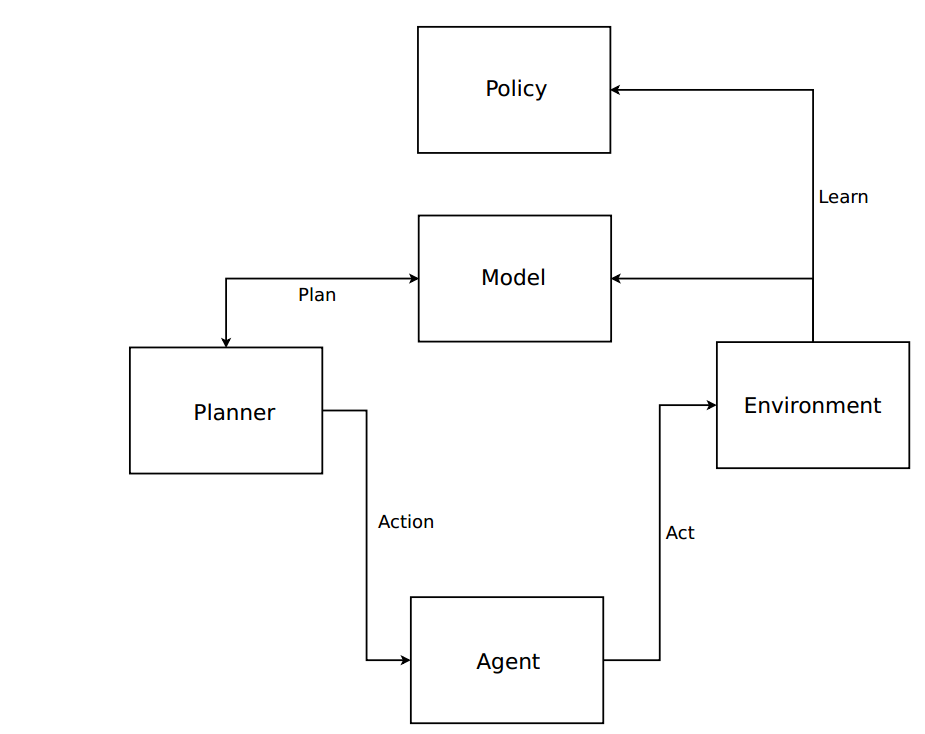
\includegraphics[max size={350pt}{350pt}]{report/assets/planning_phase.png}
    \caption{Planning Phase}
    \label{fig:planning_phase}
\end{figure}
\begin{figure}[h!]
    \centering
    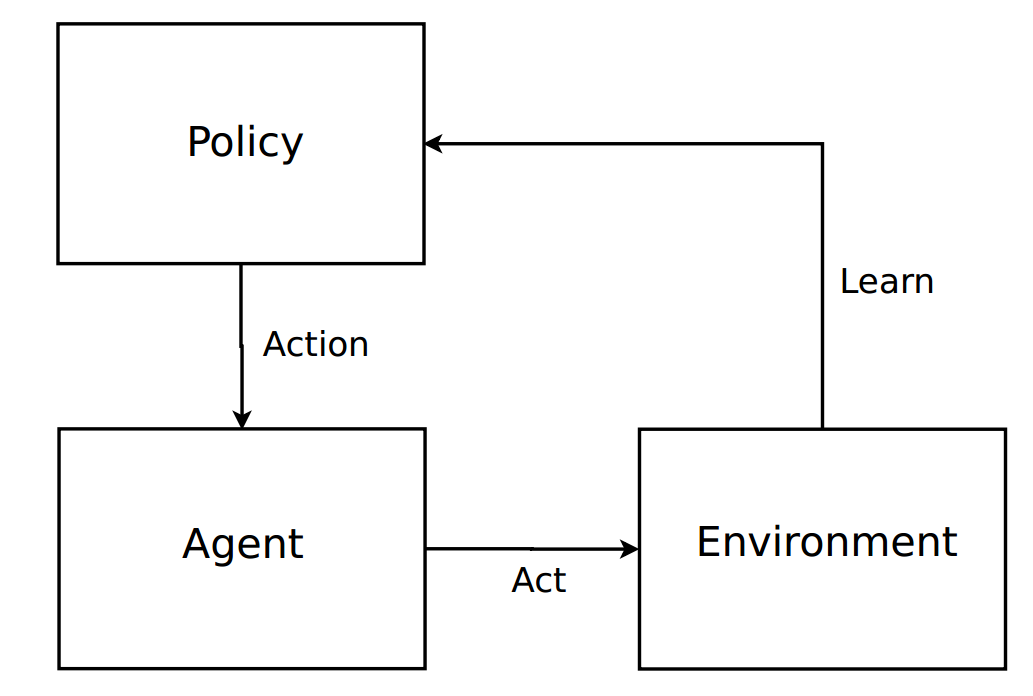
\includegraphics[max size={250pt}{250pt}]{report/assets/model_free_phase.png}
    \caption{Model-Free Phase}
    \label{fig:model_free_phase}
\end{figure}


\section{An Illustrative Example}
Consider the deterministic domain in Figure \ref{fig:cliff-real}. This is a modified version of the cliff-walking domain \cite{Sutton1998}. The red circle located at (0,0) is the agent; the goal is located in the bottom right corner, (0, 7). If the agent transitions into one of the "cliff" states, they are returned to the start state. Let's suppose that for some reason, perhaps due to changes in the environment, the agent is seeded with the inaccurate model shown in Figure \ref{fig:cliff-model}. A pure planning approach would fail, as it would continually plan a path that goes through the cliff, due to the inaccurate model. A pure model-free learning approach would probably be successful, as this is a very simple domain, however in reality domains can be much more complicated than this; which is where model-free methods begin to struggle.


% \begin{figure}
% \centering
% \begin{subfigure}{.5\textwidth}
%     \centering
%     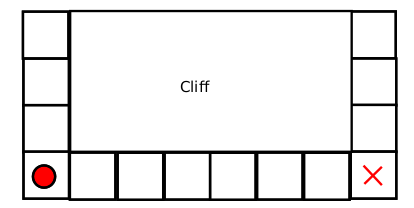
\includegraphics[max size={200}{200}]{report/assets/envs/cliff_real.png}
%     \caption{Modified Cliff-Walking Domain}
%     \label{fig:cliff-real}
% \end{subfigure}%
% \begin{subfigure}{.5\textwidth}
%   \centering
%   \includegraphics[width=.4\linewidth]{image1}
%   \caption{A subfigure}
%   \label{fig:sub2}
% \end{subfigure}
% \caption{A figure with two subfigures}
% \label{fig:test}


\begin{figure}[h!]
  \centering
  \begin{subfigure}{0.45\textwidth}
    \centering
    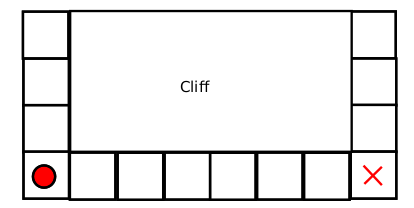
\includegraphics[max size={200}{200}]{report/assets/envs/cliff_real.png}
    \caption{Modified Cliff-Walking Domain}
    \label{fig:cliff-real}
  \end{subfigure}
  \hfill
  \begin{subfigure}{0.45\textwidth}
    \centering
    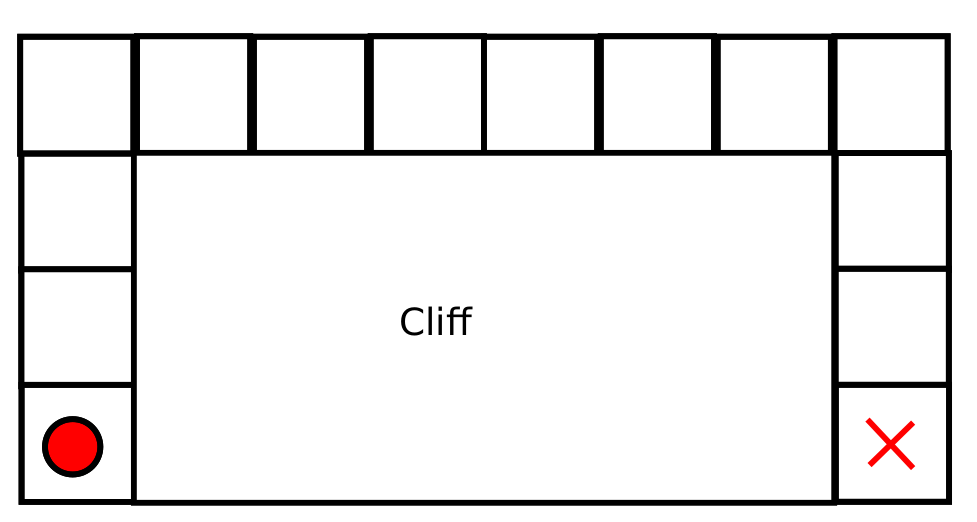
\includegraphics[max size={200}{200}]{report/assets/envs/cliff_model.png}
    \caption{Agent's Model}
    \label{fig:cliff-model}
  \end{subfigure}
  \caption{Comparison of Modified Cliff-Walking Domain and Agent's Model}
  \label{fig:cliff-comparison}
\end{figure}


\\Assuming an implementation of our framework, where reasonable Meta Actions are embedded, that allow the agent to hypothesise changes to transitions and rewards originating in the current state, and targeting an adjacent state. 
Initially, the most beneficial changes to the model would be to remove the cliff across the bottom row, as shown in Figure \ref{fig:cliff-hyp-1}. The agent then attempts to follow the plan going across the bottom of the grid, after which it realises that the hypotheses were correct. The planner may make further hypotheses which lead to the agent trying alternate paths, for instance hypothesising that the cliff is not present across the second row and that the reward through that row is increased; meaning that it would be a better path than the previous one. This process continues, with the planner making hypotheses and the agent verifying them, until no more hypotheses can be made, or the agent runs out of planning steps, after which the model-free learning takes over, and the produce policy matches the initial plan.

\begin{figure}[h!]
    \centering
    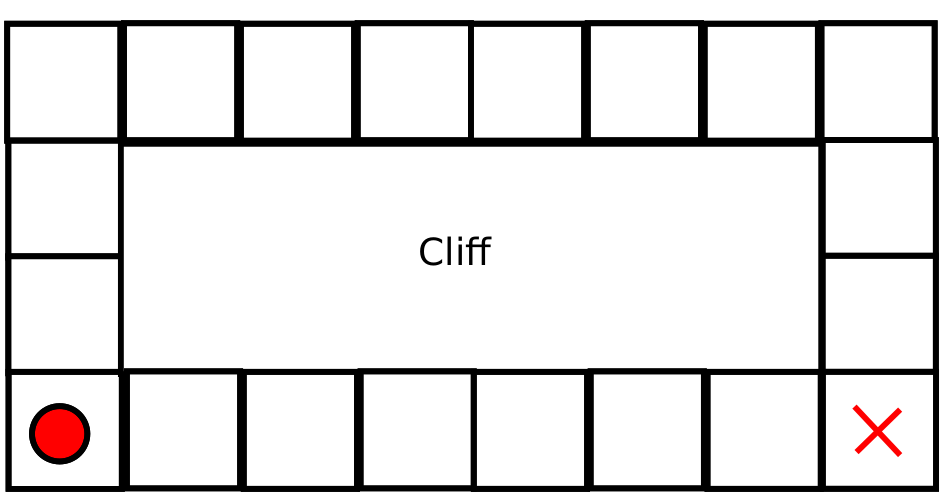
\includegraphics[max size={200}{200}]
    {report/assets/envs/cliff_hypothesis_1.png}
    \caption{Hypothesised Model}
    \label{fig:cliff-hyp-1}
\end{figure}
\section{Implementations}
The high-level ideas of the framework led to various implementations. The main differences among the implementations lie in the choice of planning algorithm, thus how the planning algorithm hypothesises changes, the available Meta Actions and the source of reasonable Meta Actions; learned versus embedded. Furthermore, some implementations had simplifications applied to them to deal with specific domains. We note that these implementations are not definitive, and much improvements could be made, but they are designed with the goal of proving the usefulness of Meta Actions. 
% All implementations were developed in Python. Whilst C or C++ would have been a better choice for computational reasons, various RL benchmarking suites are available for Python.
\subsection{RL-A* Meta}
\label{sec:rlam}
This was the initial implementation of the framework. The chosen planner was a basic A* planner, which limited the implementation to deterministic domains. A* was chosen due to ease of implementation and its use of an evaluation function, $f$, which provided a good means of evaluating Meta Actions. As discussed in Section \ref{sec:astar}, the evaluation function, $f$, is the combination of the heuristic function, $h$, and the cost function. For the cost function, it was intuitive to utilise the reward function. Namely, we define the cost of being in a state, $s$, as the sum of inverted rewards that it took to arrive at that state. Namely:
\begin{equation}
\label{eqn:astarval}
f(s_t) = -\sum_{k=0}^{t-1}\Bigg[R(s_k, a_k, s_{k+1})\Bigg] + h(s_t)
\end{equation}
The choice of heuristic, $h$, relies on domain specific knowledge, therefore we do not define it here. However,  it remains that the heuristic must be admissible. At each state, the next one to be expanded is chosen such that it maximises $f$, taking into account the Meta Actions.
\subsection{RL-A* Meta, with short term memory}
\label{sec:342}
This implementation was an extension of RL-A* Meta, which aimed to scale to stochastic domains. The stochastic nature meant that the evaluation function once again needed to be modified, as such:
\begin{equation}
\label{eqn:astarevalsast}
f(s_t) = -\sum_{k=0}^{t-1}\Bigg[(1-T(s_k, a_k, s_{k+1}))R(s_k, a_k, s_{k+1})\Bigg] + h(s_t)
\end{equation}
Since transitions were not guaranteed, the cost was weighted using the probability of the transition not occurring. This meant that transitions with a higher probability of occurring were preferred.
% \\ The Meta Actions that were available to the planner allowed it to increase/decrease transition probabilities and increase/decrease rewards for state-action-state triples. Reasonable meta actions were embedded in the model by-hand. 
To ensure feasibility of Meta Actions, a table was maintained which kept track of which actions had been called on which state-action-state triples within the previous $N$ episodes; we refer to this as the short-term memory. This encouraged the agent to try Meta Actions again that it had tried in the past, but "forgotten" that it had done so; if it got unlucky previously due to stochasticity, it could try again and discover a good policy it may not have been able to discover before.
\subsection{RL-VI Meta}
The main problem with the RL-A* agents is the reliance on a good heuristic function, which can be difficult to design and hence, they are limited to domains where a good heuristic function can be easily designed.
Therefore, this implementation aims to deal with varying domains. We opted for planning by dynamic programming, namely through Value Iteration (VI). VI was chosen because it allowed for us to easily evaluate plans through the Value Function. We chose VI over Policy Iteration, as it is generally faster, and we needed to perform it many times. Despite its nature, in our setting repeatedly performing VI is not too expensive, as real and hypothetical changes to the model are not too different, which means that it can converge in few iterations. We used a slightly modified version of VI that allowed it to evaluate the Meta Actions. Namely the updated rule was modified as such:
\begin{equation}
\label{eqn:meta_vi}
    V(s) = \max_a \sum_{s'}\max_{M'}T''(s,a,s')[R''(s,a,s') + V(s')]
\end{equation}
Where $M'=(S,A,T'',R'')$ represents each candidate MDP; this includes the original MDP, and those that can be produced by applying each Meta Action.

\subsection{RL-VI Meta, with learned Meta Actions}
The overall implementation is the same as RL-VI Meta, except Meta Actions are learned and obtained through experience, rather than embedded by-hand in the model. Meta Actions are learned when a discrepancy is noticed between the model and the real environment. For instance, when a reward is received that wasn't expected, a Meta Action is learned that increases reward to the value of the unexpected reward. Furthermore, when a transition is experienced that is unexpected, a Meta Action is learned that enables the discrepancy to be emulated; for instance, if the agent expects to move a single state vertically on an "UP" action, but it actually moves to the right, then it will learn to increase the transition probability of moving right on the "UP" action.


% A Meta Action is learned when a discrepancy is noticed between the model and the real environment. When a reward is received for a state-action-state triple that is not expected by the model, a Meta Action is learned to modify the reward function to produce this reward. When a transition occurs that is not expected by the model, a Meta Action is learned that allows the transition function to be modified elsewhere, in the same way. For example, in the Cliff-Walking domain in Figure \ref{fig:cliff-real}, the agent expects taking the "UP" action in a state to move it a single state upwards, if it actually occurs that the agent is moved two states upwards, then the agent will learn a Meta Action that enables the transition probability of moving upwards twice to be increased.


% In the context of rewards, this was as simple as adding a Meta Action for each different reward received. IN the case of transitions, if an action "UP" is taken, which the model expects to move the agent a single state in the upward direction, but actually moves the agent two states upwards, then the agent learns the Meta Action that adds a transition to move two states upwards on the "UP" action. 
\chapter{Empirical Evaluation}
\label{chapter4}
Within this chapter, we evaluate our various implementations in a collection of gridworld-like domains. The goal of the evaluation is to see how effectively our agents can explore and learn against baseline methods. 

% Furthermore, we perform some ablation studies to evaluate how important certain elements of our framework are to success. We finish by evaluating how well our agents are able to generalise to differing tasks within a domain.

\section{Baselines}
In order to truly evaluate our framework implementations, we needed some baselines to compare against. Firstly, we chose $\epsilon$-greedy, with simulated annealing, due to its ubiquity. Secondly, we chose "PRL", a model-based exploration method that always acts greedily with respect to current model during exploration, which is updated through observations; this is essentially our framework minus the Meta Actions, and is explained quite well by Algorithm \ref{alg:framework_pc}. 
This was chosen as we wanted to evaluate the usefulness of Meta Actions.

% We decided not to compare against SOTA algorithms discussed in the literature review, as due to their complexities they would prove difficult to implement. 
% Furthermore, it didn't seem like a fair comparison, as we made various simplifications when implementing our framework.

\section{Domains}
The domains that we chose to evaluate within were all gridworld-based. This decision was made due to the ease of modelling such domains, especially in a tabular manner. Furthermore, this enabled us to easily understand how the agents explore. Thus, the actions available to the agents are common between tasks (unless specified otherwise); up, down, left and right.
\\Gridworld is a deterministic domain, shown in Figure \ref{fig:grid_domain}. The agent starts in the middle of the room at the bottom of the grid. There are three doors to leave the room, in the left, right and top of the room. All of the doors are open, if they were closed then the agent would not know how to open them. The goal of the agent is to navigate to the other side of the top door. In our experiments, the model that the agents were seeded with indicated that the door leading to the goal was closed. The agent receives a reward of -1 at every time step.
\\Cliff-Walking \cite{Sutton1998} is a deterministic domain, shown in Figures \ref{fig:cliff_walking} and \ref{fig:cliff_walking_openai}. The agent starts in the bottom left corner of the grid and needs to navigate to the goal state at the bottom right of the grid. However, there is a cliff along the bottom of the grid, which the agent needs to avoid. In our experiments, the model that the agents were seeded with indicated that the cliff was bigger than it actually is; it was along the bottom two rows of the grid. The agent receives a reward of -1 at every time step, unless it steps into the cliff which induces a reward of -100 and returns the agent to the start state (without terminating the episode).
\\Windy-Gridworld \cite{Sutton1998} is a deterministic domain, shown in Figure \ref{fig:windy_gridworld} The agent starts in the left middle of the grid, and must navigate towards a goal state on the right-hand side of the grid. However, the is an upward wind within some columns which varies in strength. The wind shifts the next state upwards by the strength of the wind. In our experiments, the model that the agents were seeded with did not capture the wind. The agent receives a reward of -1 at every time step.
\\Stochastic Gridworld is the same as Gridworld, except there is some stochasticity introduced; the top door has a probability of 0.4 of being closed, within each episode. In our experiments, the model that the agents were seeded with indicated that the door leading to the goal was closed, with probability 1. The reward formulation and the actions available to the agent remain the same along with the seeded model.
\\Frozen Lake \cite{1606.01540} is a stochastic domain, shown in Figure \ref{fig:frozen_lake}. The agent must navigate from the start state in the top-left corner to the goal state in the bottom-right corner. However, the frozen lake is slippery, meaning that the agent moves in the intended direction with probability $\frac{1}{3}$ and in either of the perpendicular directions with probability $\frac{1}{3}$ each. Furthermore, there are holes where the ice has been broken or melted and entering these holes terminate the episode. The model that the agents were seeded with did not capture the slipperiness of the frozen lake, and also suggests that there is only a single path to the goal state. Rewards are sparse; reaching the goal state returns a reward of +1, whilst at all other time steps the agent receives no reward.
\\Stochastic Windy-Gridworld is the same as Windy-Gridworld, except there is stochasticity introduced;  the wind (if there is any) is stochastic. The reward formulation and the actions available to the agent remain the same along with the seeded model.

% \section{Evaluation Metrics}
% \begin{itemize}
%     \item Learning Curve
%     \item Sample efficiency? 
% \end{itemize}
\section{Results \& Analysis}
Within this section, we present results of evaluating our implementations against the aforementioned domains. All results were generated by aggregating over 20 runs, where each run produced a sliding window view, with a window size 5. Thus, each point plotted represents the average over the previous 5 episodes averaged over the 20 runs. An outlier to this was the Frozen Lake domain, where a window size of $1$ was used. These decisions were made to reduce variance in the results due to randomness, and overall produce a more robust set of results. We also plot the 95\% confidence intervals. Throughout all experiments, a discount factor of 1.0 was used, due to the episodic nature of the domains. Moreover, a learning rate of $0.6$ was used; this was tuned by-hand and turned out to produce the best results for all agents. For the model-based agents, a maximum of $10$ planning steps was allotted.
\\Figures \ref{fig:deterministic_results} and \ref{fig:stochastic_results} present the learning curves for each agent in each of the deterministic and stochastic domains, respectively. Tables \ref{table:deterministic_results} and \ref{tab:example_table} provide summaries of these results, including the minimum, mean, maximum and final rewards, as well as the standard deviation.
\\\textbf{Gridworld} \quad In the Gridworld domain, the agent that performed best on average was RL A* Meta (RLAM), closely followed by RL VI Meta (RLVIM). The poorest performing was the RL agent, which accumulated a fair amount of negative reward in the initial episodes. During the Planning phase, RLAM and RLVIM were each able to discover the optimal policy, however the formed did it much quicker. The PRL and RL VI Meta Learn (RLVIML) agents followed the exact same path throughout the planning phase, and didn't diverge from it; this was because the PRL agent didn't experience any discprencies between its model and the domain and thus didn't replan, whilst the RLVIML agent did not actually learn any Meta Actions to utilise. Each of the model-based agents suffered considerable performance decreases whilst switching to the learnt $Q$ values. All of the agents were able to discover the optimal policy within the 100 episode limit.
\\\textbf{Windy Gridworld} \quad In the Windy Gridworld domain, the RLVIM agent outperformed the others on average, although it was closely followed by the RLAM and PRL agents. The RL agent again struggled during its initial exploration, accruing large negative rewards. While the RLAM and PRL agents were able to discover the optimal policy during exploration, the RLVIM agent was not, although it seems to have explored more thoroughly since it suffered less during the switch to the model-free learning. The RLVIML agent was not successful at all; the Meta Actions that it learned somehow led to it becoming stuck in local optima during planning and unable to complete even a single episode. Interestingly, the RLAM and PRL agents were able to achieve a maximum reward of -15.0, which is in-fact optimal, however the agent performing the best in the end was the RL agent; this may be due to insufficient exploration.
\\\textbf{Cliff-Walking} \quad In the Cliff-Walking domain, the RLVIM agent was once again the best performing on average, by some distance. It seems to have performed the best during the exploratory phase; its attempts at reasoning about the environment led to it discovering the true-cliff, enabling it to avoid it later on, and thus it didn't see too much of a drop in performance when switching to model-free learning. The RL agent again struggled with its initial exploration, with its inital performance being around a factor of a 100 worst than the other agents; this is likely due to dithering, causing the agent to step into the cliff. The RLAM and PRL agents did not perform much exploration, leading to large dips in performance once again. Furthermore, the RLVIML agent wasn't successful in learning any Meta Actions, so it performed very similarly to PRL. By the final episode all agents, but the RL agent, were able to discover the optimal policy.
\\\textbf{Stochastic Gridworld}  \quad In the Stochastic Gridworld, the PRL agent performed the best on average; although it did not perform much exploration in comparison to the other agents. Compellingly, the RLVIM agent did not suffer from the performance dip witnessed in previous domains; perhaps this is because it indeed achieved sufficient exploration. The RL agent once again accumulated considerable negative reward during its initial exploration. The RLVIML and RL A* Meta short term memory (RLAM STM) agents were completely unsuccessful. Interestingly, the successful agents learned a policy that didn't use the door, although it was open more often than not.
\\\textbf{Stochastic Windy Gridworld} \quad In the Stochastic Windy Gridworld domain, the pure RL agent achieved the best performance, followed closely by the PRL agent. In this domain, the RLVIM agent accumulated more negative reward than the RL agent during their respective initial explorations. The RLVIML and RL A* Meta short term memory (RLAMSTM) agents were completely unsuccessful, again. However, the other agents learned relatively stable policies, and were able to deal with the stochasticity well.
\\\textbf{Frozen Lake} \quad In the Frozen Lake domain, the PRL agent achieved the best performance, although all of the agents performed generally poor; achieving a maximum of 3.75\% success. In this domain, the RLVIML agent outperformed RLVIM by a small margin, this is interesting and indicates that useful Meta Actions were learned. The RLAMSTM agent failed to complete a single episode.
\\In conclusion, the model-based agents generally outperformed the pure RL agent; and the Meta agent variations tended to outperform the plain PRL agent. For the most part, all of the agents were able to learn good policies with a limited number of episodes. Learning reasonable Meta Actions didn't prove to be very successful, however using embedded Meta Actions was quite successful. The RLAMSTM agent failed in every domain; this may be due to the cost function that we formulated for the agent, and it might've been more successful if we determinised the model and used our deterministic version of A* (see Section \ref{sec:rlam}). All of the model-based agents typically displayed considerable decreases in performance when switching to model-free learning - this is caused by some states having never been visited during exploration. 

% Some states are certainly not-optimal and therefore its okay not to visit them. However, it would have been much better if we found a way to avoid this performance dip.
% \\Figure \ref{fig:stochastic_results} presents the learning curves for each agent in each of the stochastic domains. We note however that the cumulative reward is plotted for the Frozen Lake domain, due to its sparse reward signal. Table \ref{tab:example_table} provides a summary of these results, including the min, mean, max, final rewards and the standard deviation in the rewards. Within the 

% \textbf{Stochastic Gridworld} domain, the best performing agent on average was the PRL agent. However, the PRL agent once again did not perform much exploration, whereas the other agents did. The RL agent again struggled during exploration, accumulating very negative rewards. Interestingly, all agents learned a policy that doesn't use the door, even though it is open more often than not. I

% n the Stochastic Windy Gridworld domain, the best performing agent on average was the RL agent, interestingly. However, while all agents struggled with the high stochasticity they were able to learn relatively stable policies. 

% Within the \textbf{Frozen Lake} domain, the PRL agent once again performed the best. Interestingly, the RLVIML agent outperformed its counterpart that does not learn Meta Actions. The RL agent was the worst performing. In general, the agents didn't perform too well in this small, but difficult domain, achieving a maximum of 3.75\% success.


% \\For the deterministic domains, we present the learning curves for each agent in each domain in Figure \ref{fig:deterministic_results}. We also present a summary of the results, including the min, max, mean and final reward, as well as the standard deviation of the rewards, in Table \ref{table:deterministic_results}.
% \\For the stochastic domains, we also present the learning curves and a summary of the results in Figure \ref{fig:stochastic_results} and Table \ref{tab:example_table} respectively.

\begin{figure}[H]
    \centering
    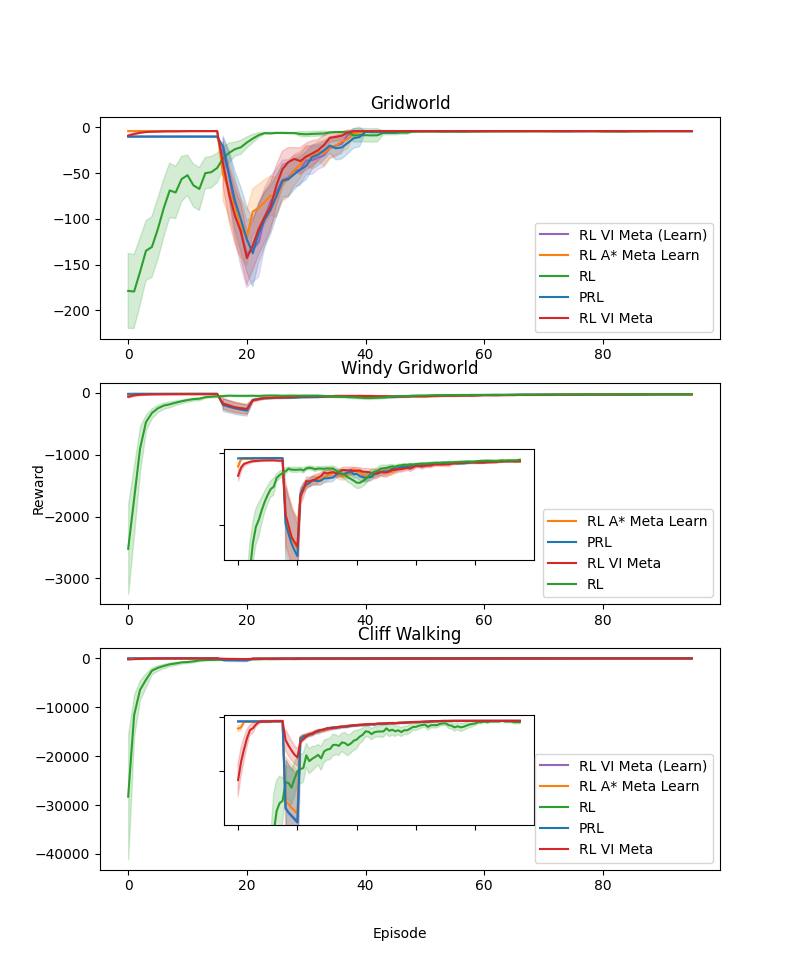
\includegraphics[max size={\textwidth}{\textheight}]{report/assets/deterministic_results.png}
    \caption{Deterministic Results}
    \label{fig:deterministic_results}
\end{figure}


\begin{figure}[H]
    \centering
    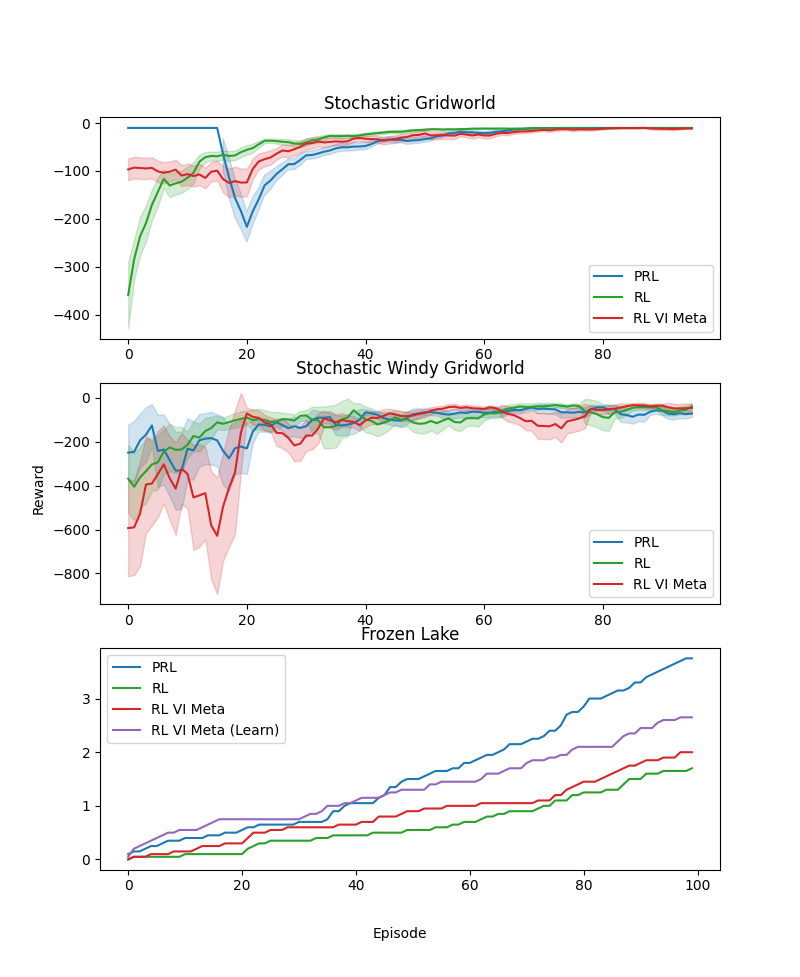
\includegraphics[max size={\textwidth}{\textheight}]{report/assets/stochastic_results.png}
    \caption{Stochastic Results}
    \label{fig:stochastic_results}
\end{figure}

\begin{table}[h]
\centering
\begin{tabular}{|c|c|c|c|}
\hline
\textbf{Agent} & \textbf{Gridworld} & \textbf{Windy Gridworld} & \textbf{Cliff-Walking}\\ \hline
\textbf{RLVIM} & 
\begin{tabular}{|c|c|}
\hline
Min & -209.72 \\ \hline
Max & -10.0 \\ \hline
Mean & -16.24 \\ \hline
Std. Dev & 29.743 \\ \hline
Final & -4.0 \\ \hline
\end{tabular}& 
\begin{tabular}{|c|c|}
\hline
Min & -259.3 \\ \hline
Max & -20.9 \\ \hline
Mean & -50.152 \\ \hline
Std. Dev & 44.944\\ \hline
Final & -23.62 \\ \hline
\hline
\end{tabular}&
\begin{tabular}{|c|c|}
\hline
Min & -231.64 \\ \hline
Max & -13.0 \\ \hline
Mean & -34.258 \\ \hline
Std. Dev & 37.456 \\ \hline
Final & -13.0 \\ \hline
\end{tabular} \\ \hline
\textbf{RLVIM (Learn)} & 
\begin{tabular}{|c|c|}
\hline
Min & -138.42 \\ \hline
Max & -4.0 \\ \hline
Mean & -18.111 \\ \hline
Std. Dev & 30.005 \\ \hline
Final & -4.0 \\ \hline
\end{tabular}& 
\begin{tabular}{|c|c|}
\hline
Min & DNF \\ \hline
Max & DNF \\ \hline
Mean & DNF \\ \hline
Std. Dev & DNF \\ \hline
Final & DNF \\ \hline
\end{tabular}& 
\begin{tabular}{|c|c|}
\hline
Min & -383.74 \\ \hline
Max & -13.0 \\ \hline
Mean & -40.66 \\ \hline
Std. Dev & 76.498 \\ \hline
Final & -13.0 \\ \hline
\end{tabular} \\ \hline
\textbf{RLAM} & 
\begin{tabular}{|c|c|}
\hline
Min & -120.58 \\ \hline
Max & -4.0 \\ \hline
Mean & -16.111 \\ \hline
Std. Dev & 26.631 \\ \hline
Final & -4.0 \\ \hline
\end{tabular}& 
\begin{tabular}{|c|c|}
\hline
Min & -267.0, \\ \hline
Max & -15.0 \\ \hline
Mean & -50.375 \\ \hline
Std. Dev & 47.226 \\ \hline
Final & -23.8 \\ \hline
\end{tabular}& 
\begin{tabular}{|c|c|}
\hline
Min & -357.08 \\ \hline
Max & -13.0 \\ \hline
Mean & -39.78 \\ \hline
Std. Dev & 70.261 \\ \hline
Final & -13.0 \\ \hline
\end{tabular} \\ \hline
\textbf{PRL} & 
\begin{tabular}{|c|c|}
\hline
Min & -137.58 \\ \hline
Max & -4.0 \\ \hline
Mean & -18.017 \\ \hline
Std. Dev & 28.838 \\ \hline
Final & -4.0 \\ \hline
\end{tabular}& 
\begin{tabular}{|c|c|}
\hline
Min & -286.64 \\ \hline
Max & -15.0 \\ \hline
Mean & -51.018 \\ \hline
Std. Dev & 51.16 \\ \hline
Final & -23.16 \\ \hline
\end{tabular}& 
\begin{tabular}{|c|c|}
\hline
Min & -388.7 \\ \hline
Max & -13.0 \\ \hline
Mean & -40.635 \\ \hline
Std. Dev & 77.127 \\ \hline
Final & -13.0 \\ \hline
\end{tabular} \\ \hline
\textbf{RL} & 
\begin{tabular}{|c|c|}
\hline
Min & -179.46 \\ \hline
Max & -4.0 \\ \hline
Mean & -21.012 \\ \hline
Std. Dev & 38.013 \\ \hline
Final & -4.06 \\ \hline
\end{tabular}& 
\begin{tabular}{|c|c|}
\hline
Min & -2521.54 \\ \hline
Max & -19.16 \\ \hline
Mean & -109.037 \\ \hline
Std. Dev &  317.461 \\ \hline
Final & -19.16 \\ \hline
\end{tabular}& 
\begin{tabular}{|c|c|}
\hline
Min & -28279.32 \\ \hline
Max & -13.2 \\ \hline
Mean & -709.696 \\ \hline
Std. Dev & 3170.597 \\ \hline
Final & -17.54 \\ \hline
\end{tabular} \\ \hline
\end{tabular}
\caption{Reward Summary for Deterministic Domains}
\label{table:deterministic_results}
\end{table}


\begin{table}[h]
\centering
\begin{tabular}{|c|c|c|c|}
\hline
\textbf{Agent} & \textbf{Stoch. Gridworld} & \textbf{Stoch. Windy Gridworld} & \textbf{Frozen Lake}\\ \hline
\textbf{RLVIM} & 
\begin{tabular}{|c|c|}
\hline
Min & -125.0 \\ \hline
Max & -9.92 \\ \hline
Mean & -44.666 \\ \hline
Std. Dev & 36.761 \\ \hline
Final & -10.92 \\ \hline
\end{tabular}& 
\begin{tabular}{|c|c|}
\hline
Min & -628.3 \\ \hline
Max & -32.9 \\ \hline
Mean & -155.688 \\ \hline
Std. Dev & 153.302\\ \hline
Final & -45.5 \\ \hline
\end{tabular}&
\begin{tabular}{|c|c|}
\hline
Success Rate & 2.0\%\\\hline
\end{tabular} \\ \hline
\textbf{RLVIM (Learn)} & 
\begin{tabular}{|c|c|}
\hline
Min & DNF\\ \hline
Max & DNF \\ \hline
Mean & DNF \\ \hline
Std. Dev & DNF \\ \hline
Final & DNF \\ \hline
\end{tabular}& 
\begin{tabular}{|c|c|}
Min & DNF \\ \hline
Max & DNF \\ \hline
Mean & DNF \\ \hline
Std. Dev & DNF \\ \hline
Final & DNF \\ \hline
\end{tabular}& 
\begin{tabular}{|c|c|}
\hline
Success Rate & 2.65\%\\\hline
\end{tabular} \\ \hline
\textbf{RLAM (STM)} & 
\begin{tabular}{|c|c|}
\hline
Min & DNF \\ \hline
Max & DNF \\ \hline
Mean & DNF \\ \hline
Std. Dev & DNF \\ \hline
Final & DNF \\ \hline
\end{tabular}& 
\begin{tabular}{|c|c|}
\hline
Min & DNF \\ \hline
Max & DNF \\ \hline
Mean & DNF \\ \hline
Std. Dev & DNF \\ \hline
Final & DNF \\ \hline
\end{tabular}& 
\begin{tabular}{|c|c|}
\hline
Success Rate & DNF\\\hline
\end{tabular} \\ \hline
\textbf{PRL} & 
\begin{tabular}{|c|c|}
\hline
Min & -216.72 \\ \hline
Max & -10.0 \\ \hline
Mean & -36.766 \\ \hline
Std. Dev & 43.71 \\ \hline
Final & -10.02 \\ \hline
\end{tabular}& 
\begin{tabular}{|c|c|}
\hline
Min & -331.2 \\ \hline
Max & -43.1 \\ \hline
Mean & -112.641 \\ \hline
Std. Dev & 70.109 \\ \hline
Final & -71.1 \\ \hline
\end{tabular}& 
\begin{tabular}{|c|c|}
\hline
Success Rate & 3.75\%\\\hline
\end{tabular} \\ \hline
\textbf{RL} & 
\begin{tabular}{|c|c|}
\hline
Min & -359.3 \\ \hline
Max & -10.22 \\ \hline
Mean & -42.7 \\ \hline
Std. Dev & 59.999 \\ \hline
Final & -10.22\\ \hline
\end{tabular}& 
\begin{tabular}{|c|c|}
\hline
Min & -405.1 \\ \hline
Max & -32.4 \\ \hline
Mean & -107.711 \\ \hline
Std. Dev &  76.601 \\ \hline
Final & -38.3 \\ \hline
\end{tabular}& 
\begin{tabular}{|c|c|}
\hline
Success Rate & 1.7\%\\\hline
\end{tabular} \\ \hline
\end{tabular}
\caption{Reward Summary for Stochastic Domains}
\label{tab:example_table}
\end{table}


% \begin{table}[h]
% \centering
% \begin{tabular}{|c|c|c|c|}
% \hline
% \textbf{Agent} & \textbf{Gridworld} & \textbf{Cliff-Walking} & \textbf{Windy Gridworld}\\ \hline
% \textbf{RLVIM} &  \hline
% \textbf{RLVIM (Learn)} & \\ \hline
% \textbf{RLAM} & \\ \hline
% \textbf{RL VI} &  \\ \hline
% \textbf{RL} &  \\ \hline
% \end{tabular}
% \caption{Reward Summary for Gridworld}
% \label{tab:example_table}
% \end{table}

% \section{Analysis}

% \section{Ablation Studies}
% \subsection{Learning from Scratch}
% \subsection{Reasonability}
% \section{Generalisation Study}

% \section{Learning from Scratch: An Ablation Study}

% \section{}

\chapter{Discussion}
\label{chapter5}

\section{Conclusion}
Exploration is a very important topic in RL, in tasks of interest its particularly important to do exploration \texit{well}; in terms of learning time and cost. Model-free exploration methods are widely used, although tend to be inefficient. An alternative is model-based exploration which often uses optimism or intrinsic motivation. Optimistic methods tend to be over-optimistic while intrinsically motivated methods rely on expensive computation. Furthermore, in most cases models are learned entirely from scratch and are assumed to eventually become correct. 
\\We proposed an approach to exploration that leverages an initial model, optimism and intrinsic motivation; whilst not relying on the model eventually becoming correct. This approach used Meta Actions, which are the main contribution of this work, which when given to a Planner enable it to hypothesise changes to the model. A framework was developed that utilises a Planner equipped with these Meta Actions to drive exploration; this framework was encapsulated in multiple implementations - the must successful of which was the RL VI Meta agent. With our empirical evaluation we showed that the use of Meta Actions can be useful in exploration, mostly under the condition of embedded reasonability, and allow our framework to overcome model inaccuracies, where it wouldn't be able to do so without; moreover, we showed that leveraging planning to drive exploration is much more sample efficient than ubiquitous model-free exploration methods such as $\epsilon$-greedy.
\\Meta Actions can be useful during exploration. We hope that this work opens the door for future research to fully understand how we can best use and learn Meta Actions.
% We applied this concept to reinforcement learning, by developing a framework that uses a planner, equipped with Meta Actions, to perform exploration. With our empirical evaluation we showed that the use of Meta Actions can be useful in exploration, and allow a model-based RL agent to overcome model inaccuracies, where it wouldn't be able to do so without; moreover, we showed that leveraging planning to drive exploration is much more sample efficient than ubiquitous model-free exploration methods such as $\epsilon$-greedy.

% both those that are embedded and those that are learned, can be useful in exploration, and allow a model-based RL agent to overcome 
% \\We conclude that Meta Actions are indeed useful, and in-fact are quite powerful in model-based exploration, and aid in overcoming model inaccuracies which allows the agent to leverage human knowledge embedded in an initial model. We believe that Meta Actions and their uses in exploration within RL is an interesting line of research, that we are interested in exploring further.
% \paragraph*{Meta Actions}
% \paragraph*{The Framework}
% \paragraph*{Evaluation}
\section{Limitations and Future Work}
The limitations of this work are mostly due to assumptions that were made to enable simplifications. Within this section we discuss these assumptions, alongside other limitations, and potential solutions as well as general ideas for future work.
% The limitations of this work are mostly due to assumptions or simplifications that were made to reduce the number of considerations needed to develop a framework that showcased our main contribution; the use of Meta Actions. Most notably, we assumed discrete (or discretised) state and action spaces, a deterministic reward function, full observability and episodic tasks. Within this section we discuss how we can reduce these assumptions along with other limitations and general ideas for future work.

\paragraph*{Stochastic Rewards and Bandits}
We assumed a deterministic reward function. This assumption is one that certainly does not hold in all domains, most notably within Bandit scenarios, where there is a single state and multiple actions \cite{lattimore}. Stochastic Rewards could be considered by extending model-learning to learn a \textit{tabular maximum likelihood model} for the reward function alongside the transition function.
\\Currently, the Meta Actions available regarding the rewards simply enable the reward to be increased. This could be modified to increase the probability of such rewards. Furthermore, in the Bandit setting, our approach of choosing when to call Meta Actions, by considering which would most benefit the planner, would probably not work; due to the single state nature, every change would most benefit the planner. Therefore in this case, a better way of choosing when to call Meta Actions needs to be considered - this could be through information theory, such as minimising uncertainty, or perhaps a count-based approach.

\paragraph*{Planning}
A key benefit of using an A* planner is that it is fast, at the cost of having to design a good, admissible, heuristic, and determinising the domain; our approach to stochasticity described in Section \ref{sec:342} was unsuccessful.  In many domains, designing a good heuristic by-hand is very difficult. However recent works, such as \cite{DBLP:journals/corr/abs-2107-02603}, have shown that heuristics can be learned directly - which is a potentially interesting extension to this work, which would allow a very simple planner to be used in perhaps a wide range of domains. However, the loss of accuracy due to determinisation could outweigh the value of decreasing computation.
\\Whilst Value Iteration natuarally deals with stochasticity, is generally slow due to its exhaustive nature, and as state spaces grow it may become very inefficient.
Furthermore, as state spaces grow, Value Iteration may become inefficient. Therefore, alternate, faster, planning algorithms, that work under stochasticity, could also be considered such as Upper Confidence Trees (UCT) \cite{10.1007/11871842_29}; which is the UCB algorithm \cite{auer2002finite} applied to tree search. 

\paragraph*{Continous State and Action Spaces}\label{p:cont}
We assumed discrete domains, or domains that offered discretisation. However, discretisation might not be sufficient; it's difficult to find a balance between coarse and fine grain state and action boundaries that maintain accuracy and efficiency. Thus, it's likely that function approximation based approaches would be a better fit for modelling. However, this introduces new issues; planning in continuous MDPs can be difficult and computationally expensive, cFVI  \cite{210504682} could be a potential option and UCT has also been extended to work in continuous state and action spaces \cite{10.1007/978-3-642-25566-3_32}.



\paragraph*{Partial Observability}
We assumed fully observable domains which is not always possible, particularly in real-life tasks of interests, such as those the robotics domain. Therefore, our approach could be extended to POMDPs, where planning would take place in belief space, rather than state space. Exactly solving POMDPs is an intractible problem, however various approaches have been suggested for approximate planning in POMDPs, such as POMCP \cite{NIPS2010_edfbe1af} and POMCPOW \cite{DBLP:journals/corr/abs-1709-06196}, the latter of which works under continuous belief and action spaces.

\paragraph*{Learning Meta Actions}
The method of learning Meta Actions that we proposed was rather simple and it wasn't vert effective during our experiments. However, we believe that learning Meta Actions is much more powerful than embedding them. An alternative approach to learning Meta Actions could leverage a Neural Network, trained through the replay buffer at the end of each episode, that takes that takes as input a state, and suggests modifications to the transitions and rewards relating to that state.

\paragraph*{Definition of Feasibility}
Whilst the definition of feasibility, given in Section \ref{sec:31}, is sufficient to prevent infinite hypothesising, through only allowing Meta Actions to be called once on a state-action pair, a stronger emphasis could be put on preventing contradictions to be made (particularly in the stochastic case, where we only consider the observations pertaining to the current episode or previous $N$ episodes). A formidable approach could be to follow the idea of \texit{known} and \texit{unknown} states, present in $E^3$ \cite{Kearns+Singh:2002} and R-MAX \cite{10.1162/153244303765208377}, only allowing Meta Actions to be called on \textit{unknown} states/state-action pairs; however this would introduce a hyperparameter, $m$, to define after how many observations a state/state-action pair becomes known.
\paragraph*{Task-Agnostic Exploration}

Our exploration approaches are goal-conditioned and task-specific. A useful line of investigation might be to consider task-agnostic exploration, where we explore the state space independent of any task, and then afterwards use extrinsic reward to adapt to downstream tasks, as in Plan2Explore \cite{plan2explore}. This could be done by choosing goals to plan and explore towards through intrinsic motivation, for instance seeking novel states that have high levels of uncertainty associated with them or seeking states with a long planning horizon. This could lead to generalisation to a variety of tasks in a given domain with minimal learning beyond the initial exploratory phase; this would take place in the model-free phase that we outlined within our framework.

\paragraph*{Further Benchmarking}
We restricted our benchmarking to gridworld-like domains. Whilst this enabled us to clearly evaluate and show the usefulness of using Meta Actions, it would have been worthwhile to benchmark our implementations in a wider range of domains, such as classic control tasks; this would've provided us with a more in-depth empirical evaluation, further showing the usefulness of our framework. Moreover, we only considered discrete tasks, it would be interesting to see how our framework performs in continuous domains (discretised, or with the modifications described pertaining to continous state and action spaces). These benchmarks could be done using OpenAI Gym \cite{1606.01540} and bsuite domains \cite{osband2020bsuite}.

\paragraph*{Beyond Episodic Tasks}
We only considered tasks with a finite time horizon associated with them. An interesting further line of work could be to consider tasks that have an infinite time horizon: continuous tasks. Task-agnostic exploration could naturally enable continuous tasks to be learned.

\paragraph*{Theoretical Analysis}
A theoretical analysis of Meta Actions would be very beneficial. In particular, we would like to prove that if there is a model inaccuracy, it will be discovered.

% \paragraph*{Continuous State and Action Spaces}
% We assumed discrete domains, or domains that offered discretisation. However, discretisation might not be sufficient; it's difficult to find a balance between coarse and fine grain state and action boundaries that maintain accuracy and efficiency. Thus, it's likely that function approximation based approaches would be a better fit, such as using Fitted Value Iteration as in \cite{SARA07-jong}.
% \paragraph*{Stochastic Rewards and Bandit Algorithms}
% Within this work, we made an assumption that rewards are deterministic. This assumption is one that certainly does not hold in most domains, most notably within Bandit scenarios, where there is a single state and multiple actions \cite{lattimore}. Stochastic Rewards could be considered by extending model-learning to learn a \textit{tabular maximum likelihood model} for the reward function alongside the transition function.
% \\Currently, the Meta Actions available regarding the rewards simply enable the reward to be increased. This could be modified to increase the probability of such rewards. Furthermore, in the Bandit setting, our approach of choosing when to call Meta Actions, by considering which would most benefit the planner, would probably not work; due to the single state nature, every change would most benefit the planner. Therefore in this case, a better way of choosing when to call Meta Actions needs to be considered - this could be through information theory, such as minimising uncertainty, or perhaps a count-based approach.
% \paragraph*{Partial Observability}
% We assumed fully observable domains which is not always possible, particularly in real-life tasks of interests, such as those the robotics domain. Therefore, our approach could be extended to POMDPs, where planning would take place in belief space, rather than state space. Exactly solving POMDPs is an intractible problem, however various approaches have been suggested for approximate planning in POMDPs, such as POMCP \cite{NIPS2010_edfbe1af}.
% \paragraph*{Planning}
% A key benefit of using an A* planner is that it is fast, at the cost of having to design a good, admissible, heuristic, and probably having to determinise the domain, although the approach to stochasticity described in Section \ref{sec:342} did work. 
% In many domains, designing a good heuristic by-hand is very difficult. However recent works, such as \cite{DBLP:journals/corr/abs-2107-02603}, have shown that heuristics for A* can be learned directly - which is a potentially interesting extension to this work, which would allow a very simple planner to be used in perhaps a wide range of domains. Furthermore, as state spaces grow, Value Iteration may become inefficient. Therefore, alternate, faster, planning algorithms could also be considered such as Upper Confidence Trees (UCT) \cite{10.1007/11871842_29}; which is the UCB algorithm \cite{auer2002finite} applied to tree search.
% \paragraph*{Task-Agnostic Exploration}
% Our exploration approaches are goal-conditioned and task-specific. A useful line of investigation might be to consider task-agnostic exploration, where we explore the state space independent of any task, and then afterwards use extrinsic reward to adapt to downstream tasks, as in Plan2Explore \cite{plan2explore}. This could be done by choosing goals to plan and explore towards through intrinsic motivation, for instance seeking novel states that have high levels of uncertainty associated with them or seeking states with a long planning horizon. This could lead to generalisation to a variety of tasks in a given domain with minimal learning beyond the initial exploratory phase; this would take place in the model-free phase that we outlined within our framework.
% \paragraph*{Beyond Episodic Tasks}
% We only considered tasks with a finite time horizon associated with them. An interesting further line of work could be to consider tasks that have an infinite time horizon: continuous tasks. Task-agnostic exploration could naturally enable continuous tasks to be learned.
% \paragraph*{Learning Meta Actions}
% The method of learning Meta Actions that we proposed is rather simple, and may not actually be that effective - a better solution might be missed out on, as a discrepancy was not experienced, and thus Meta Action learned, that allowed the it to be discovered. For example, we may learn a Meta Action that prevents a transition to take place (due to some obstacle, for instance), but we might not learn the inverse that enables us to hypothesise that an obstacle is not in-fact there, and a transition is possible. As an alternative, we may not directly learn Meta Actions but employ an "Operator" trained on experience in an environment, that takes as input a state, and suggests modifications to the transitions and rewards relating to that state.
% \paragraph*{Definition of Feasibility}
% Whilst the definition of feasibility, given in Section \ref{sec:31}, is sufficient to prevent infinite hypothesising, through only allowing Meta Actions to be called once on a SAS-triple, a stronger emphasis could be put on preventing contradictions to be made (particularly in the stochastic case, where we only consider the observations pertaining to the current episode). A formidable approach could be to follow the idea of \texit{known, unknown} and \textit{unvisited} states, present in $E^3$ \cite{Kearns+Singh:2002} and R-MAX \cite{10.1162/153244303765208377}, only allowing Meta Actions to be called on \textit{unknown} and \textit{unvisited} states/state-action pairs; however this would introduce a hyperparameter, $m$, to define after how many observations a state/state-action pair becomes known.
% \include{./report/chapters/chapter6_}

% Adds references to the table of contents.
\addcontentsline{toc}{chapter}{References}
% All your bibtex entries should go in the file called "refs.bib".
\bibliography{refs}

% All appendices you have go in a file called "appendices.tex".
\begin{appendices}

%
% The first appendix must be "Self-appraisal".
%
\chapter{Self-appraisal}

<This appendix should contain everything covered by the 'self-appraisal' criterion in the mark scheme. Although there is no length limit for this section, 2---4 pages will normally be sufficient. The format of this section is not prescribed, but you may like to organise your discussion into the following sections and subsections.>

\section{Critical self-evaluation}

\section{Personal reflection and lessons learned}

\section{Legal, social, ethical and professional issues}

<Refer to each of these issues in turn. If one or more is not relevant to your project, you should still explain {\em why} you think it was not relevant.>

\subsection{Legal issues}

\subsection{Social issues}

\subsection{Ethical issues}

\subsection{Professional issues}


%
% Any other appendices you wish to use should come after "Self-appraisal". You can have as many appendices as you like.
%
\chapter{External Material}
<This appendix should provide a brief record of materials used in the solution that are not the student's own work. Such materials might be pieces of codes made available from a research group/company or from the internet, datasets prepared by external users or any preliminary materials/drafts/notes provided by a supervisor. It should be clear what was used as ready-made components and what was developed as part of the project. This appendix should be included even if no external materials were used, in which case a statement to that effect is all that is required.>




%
% Other appendices can be added here following the same pattern as above.
%



\end{appendices}


\end{document}

